\documentclass[11pt]{report}
\usepackage[a4paper, left=2cm, right=2cm, top=2.5cm, bottom=2.5cm]{geometry}
\usepackage{theme}
\usepackage{shortcuts}

\usepackage{graphicx}
\usepackage{amsmath,amssymb}
\usepackage{booktabs}
\usepackage{float}
\usepackage{tikz}
\usetikzlibrary{positioning}

\usepackage{algorithm}
\usepackage{algorithmicx}
\usepackage{algpseudocode}

\usepackage{titlesec}
\titlespacing*{\paragraph}
  {0pt}     % left indent
  {5pt}     % space BEFORE
  {5pt}     % space AFTER

\usepackage[style=numeric]{biblatex}
\addbibresource{bibliography.bib}

% Document parameters
% Document title
\title{
      \LARGE{CentraleSupélec - Mathematics and Data Science}
      \\ \Large{Research Project Report - 2025/2026}
      \\ \large{Probabilistic Detection of Market Manipulation}
      }

\author{
      Adonis JAMAL \quad Jean-Vincent MARTINI
      \\ Supervisor: Damien CHALLET
}

\date{April 2026}

% ==============================================================================
% ================================== DOCUMENT ==================================  
% ==============================================================================
\begin{document}


% ==============================================================================
% SECTION: TITLE PAGE 
% ==============================================================================
\begin{titlepage}
\centering

{\Large CentraleSup\'elec\par}
\vspace{0.2cm}
{\large Mathematics and Data Science\par}

\vspace{1.2cm}
{\Large\bfseries Research Project Report\par}
\vspace{0.2cm}
{\large Academic Year 2025-2026\par}

\vspace{1.2cm}
{\huge\bfseries Probabilistic Detection of Market Manipulation\par}

\vspace{2.0cm}

{\large
Adonis JAMAL \quad Jean-Vincent MARTINI\par
}
\vspace{0.5cm}
{\large Supervisor: Damien CHALLET\par}
\vspace{0.2cm}
{\large Academic Tutor: Lionel GABET\par}

\vfill

{\large April 2026\par}
\vspace{1.0cm}

\begin{minipage}[c]{0.42\textwidth}
\centering

\includegraphics[height=1.8cm]{img/logoMICS.png}
\end{minipage}
\hfill
\begin{minipage}[c]{0.42\textwidth}
\centering

\includegraphics[height=1.8cm]{img/logo_cs.png}
\end{minipage}

\end{titlepage}


% ==============================================================================
% ABSTRACT
% ==============================================================================
\chapter*{Abstract}
% [CONTENT] One paragraph. State the problem (detecting spoofing, layering,
% and quote stuffing in limit order books without labelled data), the approach
% (three complementary unsupervised models with Hawkes-inspired and
% microstructural features, adaptive EVT thresholds, and interpretability
% methods), the main results (anomaly rates across time periods, cross-year
% stability, cluster structure of detected anomalies, spoofing gain estimates),
% and why they matter (first multi-model unsupervised pipeline combining
% probabilistic density estimation, robust autoencoders, and economic gain
% quantification on the same LOB dataset).
\url{https://github.com/adonis107/MDS-PDMM}


% ==============================================================================
% ACKNOWLEDGEMENTS
% ==============================================================================
\chapter*{Acknowledgements}
% [CONTENT] Thank Damien Challet for supervision and access to data, Lionel
% Gabet for academic guidance, and the Ruche HPC cluster at Universit\'e
% Paris-Saclay for GPU compute resources.


% ==============================================================================
% TABLE OF CONTENTS
% ==============================================================================
\newpage
\tableofcontents


% ==============================================================================
% CHAPTER 1: INTRODUCTION
% ==============================================================================
\chapter{Introduction}\label{chap:intro}

\section{Context and Motivation}\label{sec:intro:context}

Modern securities exchanges organise trading through electronic limit order books.
A limit order book (LOB) records all outstanding buy and sell orders at each price level, providing a real-time, public summary of supply and demand.
The instantaneous state of the book, defined by the distribution of volume across price levels on both sides, and the recent flow of incoming orders jointly determine short-term price dynamics.
Tao et al.~\cite{tao_2020} model this dependence through a multi-level volume imbalance that aggregates supply and demand across several price levels, showing on TMX data that imbalance shifts are directly linked to the probability distribution of subsequent price moves.
Fabre and Challet~\cite{fabre_2025} extend this line of work by introducing Hawkes-inspired order flow features that capture both the size and the distance of placement of new limit orders, demonstrating on cryptocurrency data that these features predict the conditional distribution of mid-price movements.

Market manipulation exploits this dependence.
By artificially altering either the instantaneous book state or the order flow, a manipulator can induce a predictable price response and profit from it.
Spoofing, the primary focus of this project, consists of placing large visible limit orders with no intention of execution.
These orders shift the perceived supply-demand balance, move the mid-price in the desired direction, and are cancelled once the manipulator's genuine order on the opposite side has been filled.
Layering extends spoofing by stacking multiple non-bona-fide orders across several price levels, amplifying the perceived depth on one side of the book~\cite{fabre_2025}.
Both strategies distort the volume imbalance: Tao et al.~\cite{tao_2020} show that the optimal spoofing action shifts the multi-level imbalance away from its equilibrium value, and that comparing the observed imbalance before a market order to its long-run distribution provides a basis for detection.

The regulatory treatment of these strategies differs sharply between asset classes.
In regulated equity and derivatives markets, spoofing and layering are explicitly prohibited under the European Market Abuse Regulation (EU MAR) and the US Dodd-Frank Act.
In cryptocurrency markets, the absence of equivalent regulation opens the door to manipulative behaviour on a larger scale~\cite{fabre_2025}.
Fabre and Challet, working on Level-3 crypto order book data, find that 31\% of large orders on the BTC-USD and ETH-USD pairs could profitably spoof the market over a four-day period.
This asymmetry suggests that crypto order book data should contain a substantially higher base rate of manipulative patterns than equity data.
The present work focuses on the more challenging equity setting, where manipulation is rarer and must be detected without labels.

\paragraph{Why unsupervised, score-based detection.}\label{sec:intro:problem}
A binary classifier that labels each event as ``manipulative'' or ``not'' is poorly suited to this detection problem for three reasons.
First, no ground-truth labels exist: in equity markets, confirmed manipulation cases are rare and not publicly annotated at the order level.
Second, manipulation is not a discrete category but a spectrum of intent, from aggressive but legitimate liquidity provision to unambiguous spoofing.
Third, a probabilistic score is more actionable than a binary flag: it allows a surveillance system to rank events by severity and calibrate alert thresholds to a desired false discovery rate.
Fabre and Challet~\cite{fabre_2025} address these requirements with a probabilistic neural network that outputs a full predictive distribution over future price moves, from which both an anomaly score (the negative log-likelihood) and an economic spoofing gain estimate (formalised in Section~\ref{sec:methodology:spoofing}) can be derived.


\section{Research Questions}\label{sec:intro:questions}

This project investigates the following questions:

\begin{enumerate}
    \item Can unsupervised probabilistic models trained on order book features detect anomalous order flow in the absence of ground-truth labels?
    \item Which order book features carry the most information about anomalous events, and do different detection models agree on the same discriminative features?
    \item How should anomaly thresholds be calibrated in a non-stationary, streaming setting when no labelled data are available?
    \item Can the economic profitability of a spoofing strategy be estimated directly from model predictions, providing an interpretable measure of manipulation opportunity?
    \item Do detection patterns remain stable across different time periods, when models trained on one year are applied to data from other years?
\end{enumerate}

These questions are addressed on the TOTF.PA (TotalEnergies, Euronext Paris) limit order book dataset, covering trading days from 2009, 2010, 2015, and 2017.


\section{Contributions}\label{sec:intro:contributions}

The main contributions of this report are:

\begin{enumerate}
    \item A modular detection pipeline that combines three complementary unsupervised models on the same equity LOB dataset (TOTF.PA, Euronext Paris): a Transformer bottleneck autoencoder inspired by Poutr\'e et al.~\cite{poutre_2024}, coupled with a Nystr\"om-approximated One-Class SVM in latent space; a Probabilistic Neural Network (PNN) that predicts skew-normal price move distributions following the framework of Fabre and Challet~\cite{fabre_2025}; and a Probabilistic Robust Autoencoder (PRAE) with learnable per-sample gates~\cite{lindenbaum2022prae}. Each model produces a scalar anomaly score per time step; their agreement identifies the highest-confidence anomalies.

    \item A feature engineering library of approximately 80 features synthesising contributions from multiple sources: Hawkes-inspired memory features with spatial and temporal decay~\cite{fabre_2025}, weighted multi-level volume imbalance~\cite{tao_2020}, event flow and cancellation rapidity~\cite{poutre_2024}, multi-level order flow imbalance, and standard microstructural indicators (spread, volatility, elasticity).
      This represents an input space roughly six times larger than that of Poutr\'e et~al.~\cite{poutre_2024}, who use approximately 13~Level-1 features.

    \item Application of the spoofing gain framework of Fabre and Challet~\cite{fabre_2025} to equity LOB data.  The PNN-predicted skew-normal parameters feed an expected cost model that quantifies the profitability of a hypothetical spoofing strategy at each time step, producing an interpretable economic measure of manipulation opportunity.

    \item A systematic comparison of four threshold methods for converting continuous anomaly scores into binary alerts without labels: Peak Over Threshold (POT), Streaming POT (SPOT), Drift-aware Streaming POT (DSPOT)~\cite{siffer:hal-01640325}, and a rolling Benjamini-Hochberg False Discovery Rate controller (RFDR).

    \item Interpretability analysis via Integrated Gradients~\cite{sundararajan2017axiomaticattributiondeepnetworks} for the PNN and PRAE, and Grouped Occlusion for the Transformer+OC-SVM, identifying which feature families and which sides of the order book drive each model's anomaly scores.

    \item Post-hoc characterisation of detected anomalies through HDBSCAN clustering of the three anomaly scores and microstructural jump analysis (bipower variation, variance ratio, CUSUM), providing an unsupervised taxonomy of anomaly types.

    \item Cross-year robustness evaluation: models trained on 2015 data are tested on 2009, 2010, and 2017 data, and models trained on 2017 data are tested on the same periods, assessing whether the pipeline detects consistent patterns across different market regimes.
\end{enumerate}


\section{Report Outline}\label{sec:intro:outline}

Chapter~\ref{chap:background} reviews the literature on limit order book microstructure, market manipulation, and the detection methods that this project builds on.
Chapter~\ref{chap:methodology} formalises the feature engineering pipeline, the three detection models with their loss functions, the threshold methods, the spoofing gain framework, and the interpretability and post-hoc analysis tools.
Chapter~\ref{chap:data} describes the TOTF.PA dataset, the preprocessing steps, the sequential training protocol, and the experimental setup.
Chapter~\ref{chap:results} presents the experimental findings: model diagnostics, anomaly detection rates, threshold comparisons, sensitivity analysis, anomaly clustering, jump analysis, and cross-year robustness.
Chapter~\ref{chap:discussion} discusses the limitations of the approach, compares the three detection models, and interprets the detected anomalies in light of known manipulation signatures.
Chapter~\ref{chap:conclusion} summarises the contributions and outlines directions for future work.


% ==============================================================================
% CHAPTER 2: BACKGROUND AND RELATED WORK
% ==============================================================================
\chapter{Background and Related Work}\label{chap:background}

This chapter provides the conceptual vocabulary and critical perspective needed to evaluate the methodological choices presented in Chapter~\ref{chap:methodology}.
Each section introduces a class of approaches, explains what it is good at, where it struggles, and what assumptions it makes.
Formal definitions, model architectures, and training procedures are deferred to Chapter~\ref{chap:methodology}.

\section{Limit Order Books and Market Microstructure}\label{sec:background:lob}

A limit order book records all outstanding buy and sell orders for a security, organised by price and submission time.
At time~$t$, the book state consists of $L$ price levels on each side.
The bid (buy) side lists prices $p^b_1 > p^b_2 > \cdots > p^b_L$ with corresponding volumes $v^b_1, v^b_2, \ldots, v^b_L$.
The ask (sell) side lists prices $p^a_1 < p^a_2 < \cdots < p^a_L$ with volumes $v^a_1, v^a_2, \ldots, v^a_L$.
The best bid is~$p^b_1$, the best ask is~$p^a_1$, the mid-price is $p_{\text{mid}} = (p^a_1 + p^b_1)/2$, and the spread is $s = p^a_1 - p^b_1$.

Three event types modify the book state.
A \emph{limit order} adds volume at a specified price level, increasing liquidity.
A \emph{cancellation} removes a previously placed limit order, reducing liquidity at that level.
A \emph{market order} (equivalently, a trade) consumes volume at the best price on the opposite side, removing liquidity and potentially shifting the best price.

The instantaneous distribution of volume across price levels and the temporal sequence of these events jointly determine short-term price dynamics.
Volume imbalance, the normalised excess of bid over ask volume at a given level, is a widely used summary statistic of the book state.
Tao et~al.~\cite{tao_2020} extend the single-level imbalance to a weighted multi-level measure that aggregates supply and demand across several price levels, and show on TMX (Toronto Stock Exchange) data that this quantity is directly linked to the probability distribution of subsequent price moves.
Fabre and Challet~\cite{fabre_2025} complement imbalance with Hawkes-inspired features that capture both the size and the spatial placement depth of new limit orders, demonstrating on cryptocurrency data that these features predict the conditional distribution of mid-price movements.

\section{Market Manipulation Strategies}\label{sec:background:manipulation}

Spoofing consists of submitting large, visible limit orders with no intention of execution to create a false impression of supply or demand.
The lifecycle of a spoofing event follows a characteristic sequence:
(1)~the manipulator places one or more large limit orders on one side of the book, shifting the perceived imbalance;
(2)~the mid-price moves in the direction favoured by the manipulator;
(3)~the manipulator executes a genuine order on the opposite side at the improved price;
(4)~the non-bona-fide orders are cancelled.
Layering extends spoofing by stacking multiple orders across several price levels on the same side, amplifying the perceived depth~\cite{fabre_2025}.
Quote stuffing is a related strategy in which a large number of orders are rapidly submitted and cancelled to flood the matching engine with messages, degrading other participants' ability to process market data and exploiting the resulting informational advantage.
Unlike spoofing, quote stuffing operates primarily through message-rate pressure rather than through direct manipulation of the perceived volume imbalance.

Both spoofing and layering are prohibited under the European Market Abuse Regulation (EU MAR, Article~12) and the US Dodd-Frank Act (Section~747).
Detection is challenging because the same order flow patterns can arise from legitimate trading strategies, such as aggressive liquidity provision or inventory management.
Tao et~al.~\cite{tao_2020} formalise the detection problem by modelling the imbalance shift caused by a spoof order and comparing the observed pre-trade imbalance distribution to its long-run counterpart via the Wasserstein distance.
Fabre and Challet~\cite{fabre_2025} take an economic approach: rather than asking whether an order flow pattern looks abnormal, they ask whether a rational spoofer could profit from the current book state, defining the spoofing gain as the difference in expected execution cost between a scenario where the spoof order is present and one where it is absent.

The arguments for unsupervised, score-based detection over binary classification are detailed in Section~\ref{sec:intro:problem} and are not repeated here.

\section{Anomaly Detection in Financial Data}\label{sec:background:anomaly}

In the absence of ground-truth labels for manipulation, detection must proceed unsupervised.
A central difficulty shared by all unsupervised approaches is the \emph{contamination problem}: training data collected from a real market inevitably contains some anomalous events, and their presence can degrade the learned model of normality.
This section surveys three families of approaches and discusses their relative strengths and weaknesses for the LOB anomaly detection problem.

\subsection{Reconstruction-Based Approaches}\label{subsec:background:reconstruction}

Autoencoders learn a compressed representation of the training data and reconstruct each input from that representation.
When the training set is predominantly normal, the model learns to reconstruct normal patterns well; anomalous inputs produce high reconstruction error because they deviate from the learned structure.
This family has several merits: it requires no labels, captures complex multivariate dependencies, and generalises across instruments and time periods without task-specific supervision.

For order book sequences, the choice of encoder architecture matters.
Convolutional and recurrent architectures capture local patterns effectively but struggle with long-range dependencies between distant price levels or between events separated by many time steps.
The Transformer architecture addresses this limitation through self-attention, which allows each position in the sequence to attend directly to every other position.
Multi-head attention enables the model to simultaneously capture different aspects of the book state, such as volume dynamics at the top of the book, spread behaviour, and order arrival patterns deeper in the queue.
Poutr\'e et~al.~\cite{poutre_2024} demonstrate on NASDAQ LOBSTER data that a Transformer autoencoder combined with a one-class classifier in the latent space outperforms the reconstruction error alone for detecting synthetically injected manipulation patterns (quote stuffing, layering, and pump-and-dump).
Notably, their feature set is built from Level-1 (best bid/ask) data only, yielding approximately 13~features; the present work extends this approach to Level-2 (ten price levels per side) data with roughly 80~features, which introduces both richer information and a substantially higher-dimensional input space.

A limitation of deterministic autoencoders is that the reconstruction error is a noisy proxy for anomaly severity: it does not distinguish between inputs that are merely unusual and inputs that fall outside the training distribution entirely.
A probabilistic formulation, in which the autoencoder outputs a distribution over reconstructions rather than a point estimate, addresses this limitation by providing an uncertainty signal.
Lindenbaum et~al.~\cite{lindenbaum2022prae} go further: rather than modifying the reconstruction itself, they introduce learnable per-sample gates that allow the training procedure to downweight suspected anomalies, so that the autoencoder focuses on reconstructing clean data even when the training set is contaminated.
This makes the model robust to the contamination problem without requiring an explicit data-cleaning step.
The degree of contamination in the specific TOTF.PA dataset is unknown; the PRAE's robustness is therefore a precautionary measure rather than a response to a measured contamination rate.

\subsection{Probabilistic Scoring via Synthetic Manipulation}\label{subsec:background:scoring}

An alternative to asking ``does this look abnormal?''\ is to ask ``how much could a rational spoofer gain from this book state?''
Fabre and Challet~\cite{fabre_2025} pursue this reframing by training a probabilistic neural network that predicts the full conditional distribution of the next mid-price move.
The predicted distribution serves two purposes: its negative log-likelihood provides a general anomaly score (events where the realised price move is unlikely under the model receive high scores), and its parameters feed an expected cost model that quantifies the profitability of a hypothetical spoofing strategy at each time step.

The merits of this approach are substantial.
The spoofing gain score has a direct economic interpretation, which makes it more actionable for a market surveillance system than a generic reconstruction error.
Training on the predictive task sidesteps the need for labelled manipulation data: the model learns normal price dynamics, and deviations from that model are flagged regardless of their cause.
The probabilistic output naturally quantifies uncertainty over the predicted price move, which matters for heavy-tailed financial data where point predictions are unreliable.

The limitations are equally clear.
The spoofing gain depends on a model of the spoofer's strategy (order size, placement distance, fee structure), so it may miss manipulation patterns that deviate from that model.
The approach was developed and evaluated on cryptocurrency LOB data (BTC-USD and ETH-USD on Coinbase)~\cite{fabre_2025}, where the absence of anti-manipulation regulation results in a higher base rate of manipulative behaviour; its effectiveness on regulated equity markets, where manipulation is rarer and subtler, has not been established in the literature.

\subsection{One-Class and Density-Based Approaches}\label{subsec:background:oneclass}

One-class classification methods learn a tight boundary around the training data in a transformed feature space and flag anything outside that boundary as anomalous.
The One-Class SVM (OC-SVM) is the most widely used instance: it finds a hyperplane in a kernel-induced feature space that separates the data from the origin with maximum margin, controlled by a parameter $\nu$ that bounds the fraction of training points allowed outside the boundary.

The strengths of the OC-SVM are computational efficiency and theoretical simplicity.
It does not require specifying what an anomaly looks like, only what normal data looks like, and the kernel trick allows it to capture non-linear structure in the input space.
However, it does not scale well to high-dimensional feature spaces without careful kernel design: in the approximately 80-dimensional feature space typical of LOB anomaly detection, the RBF kernel becomes poorly calibrated and the decision boundary may either collapse or become too loose.
Low-rank kernel approximations (such as the Nystr\"om method) partially address this issue by projecting the kernel evaluation into a tractable subspace, enabling GPU-accelerated training.
A further limitation is that the OC-SVM does not produce a calibrated probability; its decision function is a signed distance, not a likelihood, which complicates downstream interpretation and threshold calibration.

For the LOB problem, the OC-SVM is most effective when applied not to raw features but to a learned latent representation.
Poutr\'e et~al.~\cite{poutre_2024} demonstrate this by fitting an OC-SVM in the bottleneck space of a Transformer autoencoder, where the reduced dimensionality and the learned structure of the representation make the kernel boundary more discriminative.
This two-stage approach combines the representation power of reconstruction-based methods with the boundary-learning capacity of one-class classification.

\section{Thresholding Methods for Anomaly Detection}\label{sec:background:thresholding}

Any continuous anomaly score requires a threshold to produce a detection decision.
The naive approach, a fixed percentile of the score distribution, assumes that the distribution is stationary and well-behaved.
In financial data, score distributions are heavy-tailed and non-stationary: a fixed percentile will produce too many false positives during volatile periods and miss anomalies during quiet periods.
Setting thresholds without labels is therefore a problem in its own right.

\paragraph{Extreme Value Theory (EVT).}
EVT models the tail of the score distribution rather than the bulk, fitting a Generalised Pareto Distribution to the exceedances above a high initial threshold.
This is well-suited to heavy-tailed data because the statistical guarantee applies specifically to extreme quantiles, where fixed-percentile methods are least reliable.
Siffer et~al.~\cite{siffer:hal-01640325} extend the batch EVT estimator to streaming settings with two algorithms: SPOT, which updates the tail model as new peaks arrive, and DSPOT, which adds a drift correction that tracks shifts in the baseline score level over time.
The main assumption is that the tail of the score distribution is well-approximated by the GPD, which must be verified empirically for each model output.

\paragraph{False Discovery Rate (FDR) Control.}
FDR-based procedures, such as the Benjamini-Hochberg method, control the expected proportion of false positives among all flagged events.
This is appropriate when anomalies are rare and the cost of false positives is high, because it bounds the discovery error rate rather than the absolute false positive count.
The requirement is a set of p-values or a reference null distribution for the anomaly score, which must be estimated from the data when no parametric form is available.

\paragraph{Rolling FDR (RFDR).}
RFDR adapts the Benjamini-Hochberg procedure to a streaming setting by maintaining a sliding window of recent anomaly scores.
Within each window, scores are log-transformed, converted to robust z-scores using the median absolute deviation, and mapped to p-values under a Gaussian assumption; the BH procedure then determines a dynamic threshold that controls the false discovery rate at level~$\alpha$.
Because the null distribution is re-estimated at every step from the local window, RFDR tracks non-stationarity in the score distribution without requiring an explicit drift model.

\paragraph{Implicit and Post-Hoc Model Thresholds.}
Some detection methods appear to produce a threshold as a byproduct of training.
The OC-SVM decision boundary, for instance, defines a binary classification in the feature space: points with negative decision function values are labelled as outliers.
However, in practice this binary output is often discarded in favour of a continuous dissimilarity score, and a separate threshold is selected post-hoc on labelled evaluation data.
Poutr\'e et~al.~\cite{poutre_2024} follow this approach, choosing the threshold that maximises the $F_4$-score on a test set containing synthetic manipulations.
This converts an ostensibly unsupervised method into one that depends on labelled data for threshold calibration.

\section{Feature Attribution Methods}\label{sec:background:attribution}

A detection score alone is not actionable for a market surveillance analyst: the analyst needs to know which features of the order book drove the score and whether those features align with known manipulation signatures.
Attribution for sequential financial data is harder than for static inputs because features at different time steps and price levels are structurally correlated, and because the underlying distribution shifts over the trading day.

Two broad families of attribution methods are relevant.
Gradient-based methods, such as Integrated Gradients~\cite{sundararajan2017axiomaticattributiondeepnetworks}, accumulate the model's gradient along a path from a baseline input to the actual input, producing per-feature importance scores that are theoretically principled (they satisfy completeness and sensitivity axioms) and computationally tractable.
Their limitation is that they require a differentiable end-to-end model, which excludes pipelines where a non-differentiable component (such as an OC-SVM) sits between the learned representation and the final score.

For non-differentiable pipelines, ablation-based methods provide an alternative.
Grouped occlusion replaces semantically related groups of features (all bid-side features, all Hawkes features, all features at a given price level) with a baseline value and measures the resulting change in the anomaly score.
This approach is model-agnostic and handles the structured correlation among LOB features by operating at the group level rather than the individual feature level.
The trade-off is lower resolution: it identifies which feature families matter, not which individual features within a family are most important.


% ==============================================================================
% CHAPTER 3: METHODOLOGY
% ==============================================================================
\chapter{Methodology}\label{chap:methodology}
% [CONTENT] Full formal description of the pipeline: data $\to$ features
% $\to$ model $\to$ score $\to$ threshold $\to$ alert. Each section defines
% the mathematical objects, the loss functions, and justifies design choices.

% DONE (D2.1): Pipeline diagram inserted.

\begin{figure}[H]
\centering
\resizebox{\textwidth}{!}{%
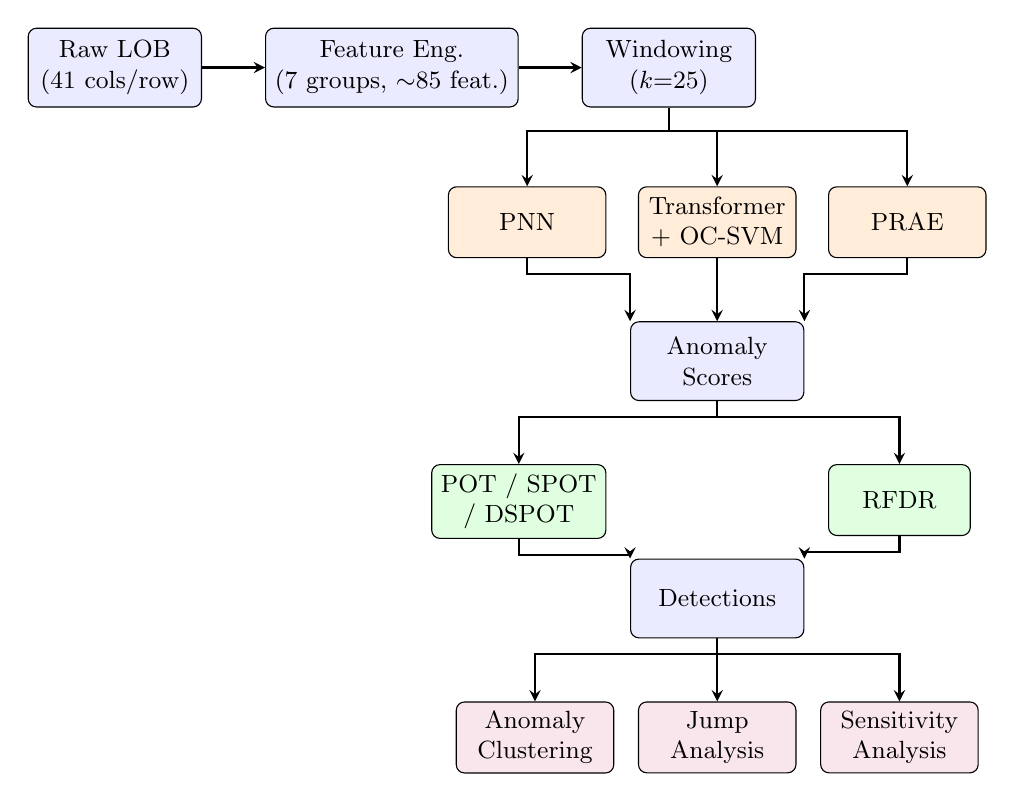
\begin{tikzpicture}[
  node distance=0.6cm and 0.8cm,
  stage/.style={rectangle, draw, rounded corners=3pt, minimum height=1cm, minimum width=2.2cm,
                align=center, font=\small, fill=blue!8},
  model/.style={rectangle, draw, rounded corners=3pt, minimum height=0.9cm, minimum width=2cm,
                align=center, font=\small, fill=orange!15},
  threshold/.style={rectangle, draw, rounded corners=3pt, minimum height=0.9cm, minimum width=1.8cm,
                    align=center, font=\small, fill=green!12},
  posthoc/.style={rectangle, draw, rounded corners=3pt, minimum height=0.9cm, minimum width=2cm,
                  align=center, font=\small, fill=purple!10},
  arr/.style={->, thick, >=stealth},
]
  % Row 1: Data pipeline
  \node[stage] (raw) {Raw LOB\\(41 cols/row)};
  \node[stage, right=of raw] (feat) {Feature Eng.\\(7 groups, ${\sim}85$ feat.)};
  \node[stage, right=of feat] (win) {Windowing\\($k{=}25$)};

  % Row 2: Models
  \node[model, below right=1.0cm and -1.5cm of win] (tfocsvm) {Transformer\\+ OC-SVM};
  \node[model, left=0.4cm of tfocsvm] (pnn) {PNN};
  \node[model, right=0.4cm of tfocsvm] (prae) {PRAE};

  % Row 3: Scores
  \node[stage, below=0.8cm of tfocsvm] (scores) {Anomaly\\Scores};

  % Row 4: Thresholding
  \node[threshold, below left=0.8cm and 0.3cm of scores] (evt) {POT / SPOT\\/ DSPOT};
  \node[threshold, below right=0.8cm and 0.3cm of scores] (rfdr) {RFDR};

  % Row 5: Detections
  \node[stage, below=0.8cm of scores, yshift=-1.2cm] (det) {Detections};

  % Row 6: Post-hoc
  \node[posthoc, below left=0.8cm and 0.2cm of det] (clust) {Anomaly\\Clustering};
  \node[posthoc, below=0.8cm of det] (jump) {Jump\\Analysis};
  \node[posthoc, below right=0.8cm and 0.2cm of det] (ig) {Sensitivity\\Analysis};

  % Arrows
  \draw[arr] (raw) -- (feat);
  \draw[arr] (feat) -- (win);
  \draw[arr] (win.south) -- ++(0,-0.3) -| (pnn.north);
  \draw[arr] (win.south) -- ++(0,-0.3) -| (tfocsvm.north);
  \draw[arr] (win.south) -- ++(0,-0.3) -| (prae.north);
  \draw[arr] (pnn.south) -- ++(0,-0.2) -| (scores.north west);
  \draw[arr] (tfocsvm.south) -- (scores.north);
  \draw[arr] (prae.south) -- ++(0,-0.2) -| (scores.north east);
  \draw[arr] (scores.south) -- ++(0,-0.2) -| (evt.north);
  \draw[arr] (scores.south) -- ++(0,-0.2) -| (rfdr.north);
  \draw[arr] (evt.south) -- ++(0,-0.2) -| (det.north west);
  \draw[arr] (rfdr.south) -- ++(0,-0.2) -| (det.north east);
  \draw[arr] (det.south) -- ++(0,-0.2) -| (clust.north);
  \draw[arr] (det.south) -- (jump.north);
  \draw[arr] (det.south) -- ++(0,-0.2) -| (ig.north);
\end{tikzpicture}%
}
\caption{End-to-end detection pipeline. Raw LOB snapshots are transformed into ${\sim}85$ features, windowed into sequences of length $k{=}25$, and scored by three complementary models. Threshold methods produce binary detections, which are analysed post hoc via clustering, jump tests, and integrated-gradient attribution.}
\label{fig:pipeline}
\end{figure}

\section{Feature Engineering}\label{sec:methodology:features}

The raw limit order book data for TOTF.PA (TotalEnergies, Euronext Paris) records the state of the book at each update event during continuous trading hours (09:00-17:30 CET).
Each row contains an Excel serial timestamp $t$ (column \texttt{xltime}, where the fractional part encodes the time of day) and the price and volume at $L = 10$ levels on each side: $p^b_1, V^b_1, \ldots, p^b_{10}, V^b_{10}$ for the bid and $p^a_1, V^a_1, \ldots, p^a_{10}, V^a_{10}$ for the ask, giving 41 columns per row.
The data is event-driven: a new row is recorded whenever a limit order, cancellation, or trade modifies the visible book state, so the inter-event spacing is irregular.

Feeding the 40 raw price-volume columns directly to a model is wasteful and fragile.
Prices at adjacent levels are highly correlated, volumes are non-stationary, and the absolute price level carries no information about short-term dynamics.
Engineered features reduce the input dimensionality to $d_{\text{in}} \approx 80$ informative quantities that are more stationary, more interpretable, and encode the domain knowledge needed to distinguish normal from anomalous order flow.

The features are organised into seven groups: (1)~order book imbalance, capturing supply-demand asymmetry across depth levels; (2)~price dynamics and microstructure, summarising price movements and their relationship to volume; (3)~liquidity and elasticity, measuring the cost and shape of the book; (4)~volatility proxies; (5)~event flow and rapidity, characterising the intensity and type of order arrivals; (6)~Hawkes-inspired memory features, capturing self-exciting patterns in order flow with spatial and temporal decay; and (7)~order flow imbalance, measuring signed directional pressure from volume changes conditioned on price movements.
Preprocessing and scaling are described in Section~\ref{subsec:features:preprocessing}.


\subsection{Order Book Imbalance}\label{subsec:features:imbalance}

Imbalance features quantify the asymmetry between supply and demand at various depths of the book.
Spoofing and layering distort this asymmetry by injecting volume on one side; imbalance measures are therefore among the most direct indicators of manipulative intent.

The Level-1 imbalance compares bid and ask volume at the best quotes:
\begin{equation}
  \label{eq:l1_imbalance}
  I^{(1)}_t = \frac{V^b_{1,t} - V^a_{1,t}}{V^b_{1,t} + V^a_{1,t}}.
\end{equation}
Values near $+1$ indicate strong buy-side pressure; values near $-1$ indicate sell-side pressure.

The Level-5 imbalance aggregates volume across the top five levels on each side:
\begin{equation}
  \label{eq:l5_imbalance}
  I^{(5)}_t = \frac{\sum_{i=1}^{5} V^b_{i,t} - \sum_{i=1}^{5} V^a_{i,t}}{\sum_{i=1}^{5} V^b_{i,t} + \sum_{i=1}^{5} V^a_{i,t}}.
\end{equation}
A divergence between $I^{(1)}_t$ and $I^{(5)}_t$ suggests that volume is concentrated away from the best quotes, a pattern consistent with layering.

To weight deeper levels more flexibly, we follow Tao et~al.~\cite{tao_2020} and define a weighted multi-level imbalance over $L = 5$ levels with weight vector $\mathbf{w} = (w_1, \ldots, w_5)$:
\begin{equation}
  \label{eq:weighted_imbalance}
  I^{(\mathbf{w})}_t = \frac{\sum_{i=1}^{5} w_i \, V^b_{i,t}}{\sum_{i=1}^{5} w_i \, V^b_{i,t} + \sum_{i=1}^{5} w_i \, V^a_{i,t}}.
\end{equation}
This quantity lies in $[0, 1]$; values above $0.5$ indicate net bid-side weight.
Three weight configurations are used: \emph{deep-weighted} $\mathbf{w} = (0.1, 0.1, 0.2, 0.2, 0.4)$, which emphasises deeper levels where spoof orders are less likely to be executed; \emph{top-weighted} $\mathbf{w} = (0.4, 0.2, 0.2, 0.1, 0.1)$, which emphasises the best quotes; and \emph{uniform} $\mathbf{w} = (0.2, 0.2, 0.2, 0.2, 0.2)$, which weights all five levels equally.
Unlike the Level-1 volume imbalance used by Poutr\'e et~al.~\cite{poutre_2024}, this weighted formulation aggregates information across five price levels, so $I^{(\mathbf{w})}_t$ reflects the depth structure of the book rather than only the best quotes.


\subsection{Price Dynamics and Microstructure}\label{subsec:features:price}

This group captures the immediate state of the price process and its first- and second-order dynamics.

The mid-price and bid-ask spread are:
\begin{equation}
  \label{eq:midprice}
  p_{\text{mid},t} = \frac{p^a_{1,t} + p^b_{1,t}}{2}, \qquad
  s_t = p^a_{1,t} - p^b_{1,t}.
\end{equation}

The micro-price deviation measures how far the L1-imbalance-adjusted fair value lies from the mid-price:
\begin{equation}
  \label{eq:microprice_deviation}
  \delta_t^{\text{micro}} = I^{(1)}_t \cdot \frac{s_t}{2}.
\end{equation}
A large deviation suggests that the balance of volume at the best quotes is pulling the fair value away from the geometric centre of the spread.

The volume depth ratio measures the concentration of volume away from the best quote on each side $s \in \{b, a\}$:
\begin{equation}
  \label{eq:depth_ratio}
  D^s_t = \frac{\sum_{i=2}^{5} V^s_{i,t}}{V^s_{1,t}}.
\end{equation}
High values indicate that most liquidity sits behind the best quote, a signature of layering where large volumes are placed at deeper levels.

Log returns, velocity, and acceleration of the mid-price are:
\begin{equation}
  \label{eq:log_return}
  r_t = \ln\!\left(\frac{p_{\text{mid},t}}{p_{\text{mid},t-1}}\right), \quad
  v_t = p_{\text{mid},t} - p_{\text{mid},t-1}, \quad
  a_t = v_t - v_{t-1}.
\end{equation}

The net order flow at Level~1 isolates volume changes that occur at a fixed price, filtering out changes caused by price-level shifts:
\begin{equation}
  \label{eq:net_flow}
  F^s_t = \Delta V^s_{1,t} \cdot \mathbf{1}\!\left[p^s_{1,t} = p^s_{1,t-1}\right], \qquad s \in \{b, a\},
\end{equation}
where $\Delta V^s_{1,t} = V^s_{1,t} - V^s_{1,t-1}$.
A large positive $F^b_t$ followed by a rapid cancellation is a textbook spoofing pattern.

Volume deltas $\Delta V^b_{1,t}$ and $\Delta V^a_{1,t}$ at the best quotes are also retained as raw features, along with the rolling standard deviation of the mid-price over a window of $W = 50$ events.


\subsection{Liquidity and Elasticity}\label{subsec:features:liquidity}

These features describe how much it costs to execute a given order size and how steeply the book's price schedule rises with volume.

The sweep-to-fill cost is the volume-weighted average price paid to execute a target order of size $Q = 1{,}000$ units by walking through $L = 10$ levels.
The value $Q = 1{,}000$ was chosen empirically to represent a moderately sized institutional order for TOTF.PA; no reference paper prescribes a specific target size, and a sensitivity analysis over $Q$ is deferred to Chapter~\ref{chap:results}.
Denoting by $C^s_t(Q)$ the resulting average execution price on side $s$, the reported features are the excess costs relative to the mid-price:
\begin{equation}
  \label{eq:sweep_cost}
  \text{SC}^a_t = C^a_t(Q) - p_{\text{mid},t}, \qquad
  \text{SC}^b_t = p_{\text{mid},t} - C^b_t(Q).
\end{equation}
Both quantities are non-negative under normal conditions.
Large values indicate thin liquidity: a spoofing episode that removes genuine orders from the book can cause a spike in sweep cost.

The book slope (elasticity) measures the sensitivity of price to cumulative volume.
For each side $s$, a linear regression of price on log cumulative volume across the first $D = 5$ levels gives the following relationship (Tao et~al.~\cite{tao_2020} calibrate a comparable depth parameter to values between 3 and 5 depending on the stock; Fabre and Challet~\cite{fabre_2025} use $K = 5$ as a representative depth):
The depth $D = 5$ is consistent with the range used by Tao et~al.~\cite{tao_2020} (who calibrate 3 to 5 depending on the stock) and Fabre and Challet~\cite{fabre_2025} (who use $K = 5$); an ablation over $D$ is reported in Chapter~\ref{chap:results}.
\begin{equation}
  \label{eq:book_slope}
  p^s_{i,t} \approx \alpha^s_t + \beta^s_t \ln\!\left(\sum_{j=1}^{i} V^s_{j,t} + 1\right), \qquad i = 1, \ldots, D,
\end{equation}
and the feature is the absolute slope $|\beta^s_t|$.
A steep slope (large $|\beta^s_t|$) indicates low liquidity, where a small volume would cause a large price change; a flat slope indicates a deep, resilient book.


\subsection{Volatility}\label{subsec:features:volatility}

Local volatility features capture the recent variability of the price process and of event timing.

Rolling standard deviations of log returns are computed over two horizons:
\begin{equation}
  \label{eq:rolling_vol}
  \sigma^{(W)}_t = \sqrt{\frac{1}{W-1}\sum_{k=0}^{W-1}(r_{t-k} - \bar{r}_t)^2}, \qquad W \in \{50, 100\}.
\end{equation}

The normalised price range over a window of $W = 50$ events measures extreme movements:
\begin{equation}
  \label{eq:price_range}
  R_t = \frac{\max_{k \in [t-W+1, t]} p_{\text{mid},k} - \min_{k \in [t-W+1, t]} p_{\text{mid},k}}{p_{\text{mid},t}}.
\end{equation}
A sudden spike in $R_t$ without a corresponding increase in $\sigma^{(50)}_t$ may indicate a transient price dislocation caused by manipulation.

The absolute velocity $|r_t|$ captures the instantaneous magnitude of price movement without directional information.

The inter-event time $\Delta t_t = t - t_{t-1}$ (in fractions of a day, following the Excel \texttt{xltime} convention) and its logarithm $\ln(\Delta t_t + \epsilon)$, with $\epsilon = 10^{-6}$, are included to provide the models with information about event timing.
Abnormally short inter-event times can signal quote-stuffing activity.


\subsection{Event Flow and Rapidity}\label{subsec:features:eventflow}

Following Poutr\'e et~al.~\cite{poutre_2024}, each LOB update is classified as either a cancellation or a trade based on observable price and volume changes.
A cancellation on side $s$ is identified when the best price is unchanged and volume decreases ($p^s_{1,t} = p^s_{1,t-1}$ and $\Delta V^s_{1,t} < 0$).
A trade on side $s$ is labelled by the \emph{aggressor} (the marketable order that initiates the transaction): a buy trade is detected when the ask price changes ($p^a_{1,t} \neq p^a_{1,t-1}$), and a sell trade when the bid price changes ($p^b_{1,t} \neq p^b_{1,t-1}$).
The corresponding event-size features are indexed by the \emph{passive} side of the book that absorbed the order ($s = b$ for a buy trade, $s = a$ for a sell trade).

The event size features record the magnitude of each event type:
\begin{equation}
  \label{eq:event_size}
  \text{Size}_t^{\text{cancel},s} = |\Delta V^s_{1,t}| \cdot \mathbf{1}[\text{cancel}^s_t], \qquad
  \text{Size}_t^{\text{trade},s} = V^s_{1,t-1} \cdot \mathbf{1}[\text{trade}^s_t].
\end{equation}
Each of these four quantities, along with the raw Level-1 volume, is smoothed with a simple moving average over $W_{\text{SMA}} = 10$ events, following the feature definitions in Poutr\'e et~al.~\cite{poutre_2024}.
The window size $W_{\text{SMA}} = 10$ follows the implementation of Poutr\'e et~al.~\cite{poutre_2024}, who adopt this value without ablation; we retain it unchanged and note that no sensitivity analysis over $W_{\text{SMA}}$ is performed in this work.

Rapidity features measure the density of events per unit of calendar time:
\begin{equation}
  \label{eq:rapidity}
  \rho_t^{\text{type},s} = \frac{\mathbf{1}[\text{type}^s_t]}{\Delta t_t}, \qquad \text{type} \in \{\text{cancel}, \text{trade}\}, \quad s \in \{b, a\}.
\end{equation}
High cancellation rapidity on one side of the book is a signature of quote stuffing, where a manipulator floods the exchange with rapid submissions and cancellations.

Bid- and ask-side log returns ($\ln(p^s_{1,t} / p^s_{1,t-1})$ for $s \in \{b, a\}$) and price speed (log return divided by $\Delta t_t$) complete this group.


\subsection{Hawkes-Inspired Memory Features}\label{subsec:features:hawkes}

Following Fabre and Challet~\cite{fabre_2025}, we define order flow variables inspired by the self-exciting structure of Hawkes processes.
Let $(N^{L,b}_t)_{t \geq 0}$ and $(N^{L,a}_t)_{t \geq 0}$ denote the point processes counting the arrivals of buy and sell limit orders, and let $(N^{M,b}_t)_{t \geq 0}$ and $(N^{M,a}_t)_{t \geq 0}$ denote the point processes of buy and sell marketable orders respectively (using the aggressor-side convention: $N^{M,b}$ counts buy market orders that consume ask-side liquidity, and $N^{M,a}$ counts sell market orders that consume bid-side liquidity).
Each limit order carries two marks: a volume $v^{L,s}_t > 0$ and a distance of placement $\delta^{L,s}_t > 0$ from the best price, for $s \in \{b, a\}$.
Each marketable order carries a volume mark $v^{M,s}_t > 0$.

The limit-order and marketable-order flow variables are defined as
\begin{equation}
  \label{eq:limit_flow}
  L^s_t(\phi) = \int_{(-\infty,t]} \phi(t - u,\, v^{L,s}_u,\, \delta^{L,s}_u)\, dN^{L,s}_u, \qquad s \in \{b, a\},
\end{equation}
\begin{equation}
  \label{eq:market_flow}
  M^s_t(\psi) = \int_{(-\infty,t]} \psi(t - u,\, v^{M,s}_u)\, dN^{M,s}_u, \qquad s \in \{b, a\},
\end{equation}
where $\phi$ is a positive kernel that weights each past limit order by its elapsed time, volume, and distance of placement, and $\psi$ is a positive kernel that weights each past marketable order by its elapsed time and volume.

The kernels take exponential form with a linear volume function $f(v) = v$:
\begin{equation}
  \label{eq:limit_kernel}
  \phi_{\beta,\eta}(t, v, \delta) = e^{-\beta t}\, v\, e^{-\eta \delta}, \qquad
  \psi_{\beta}(t, v) = e^{-\beta t}\, v,
\end{equation}
where $\beta > 0$ controls the temporal decay rate and $\eta \geq 0$ controls the spatial decay rate.
The exponential time kernel is chosen for two reasons: it satisfies the Markov property, which permits efficient recursive updates in a streaming setting, and combining multiple time scales $\beta$ approximates the slowly decaying empirical memory of order flow across several decades~\cite{fabre_2025}.

Two families of kernels are constructed by varying $\beta$ over a finite set $\boldsymbol{\beta}$ and $\eta$ over a finite set $\boldsymbol{\eta}$:
\begin{equation}
  \label{eq:kernel_families}
  \boldsymbol{\phi} = \{\phi_{\beta,\eta} : \beta \in \boldsymbol{\beta},\, \eta \in \boldsymbol{\eta}\}, \qquad
  \boldsymbol{\psi} = \{\psi_{\beta} : \beta \in \boldsymbol{\beta}\}.
\end{equation}
The corresponding feature sets at time $t$ are
\begin{equation}
  \label{eq:feature_families}
  \mathcal{L}_t = \bigl\{(L^b_t(\phi),\, L^a_t(\phi)) : \phi \in \boldsymbol{\phi}\bigr\}, \qquad
  \mathcal{M}_t = \bigl\{(M^b_t(\psi),\, M^a_t(\psi)) : \psi \in \boldsymbol{\psi}\bigr\}.
\end{equation}
Each element of $\mathcal{L}_t$ captures limit-order flow at a specific combination of time and distance scales; each element of $\mathcal{M}_t$ captures marketable-order flow at a specific time scale.
Small $\eta$ values give nearly equal weight to orders at all depths; large $\eta$ values concentrate attention on orders near the best quotes, so that distant spoof orders receive negligible weight.

\paragraph{Adaptation to Level-2 data.}
Fabre and Challet~\cite{fabre_2025} work with Level-3 data, where each order event is individually observed with its volume and distance of placement.
Our dataset provides Level-2 snapshots (aggregate volume at each of $L = 10$ price levels), so the integrals in Equations~\eqref{eq:limit_flow}-\eqref{eq:market_flow} are approximated as follows.
At each event $t$, the limit-order volume at level $i$ on side $s$ is inferred from positive volume changes at unchanged price levels: $[\Delta V^s_{i,t}]^{+} \cdot \mathbf{1}[p^s_{i,t} = p^s_{i,t-1}]$.
The distance mark $\delta^{L,s}_{i,t}$ is set to $c \cdot |p^s_{i,t} - p_{\mathrm{mid},t}|$, where $c = 10^4$ converts Euro-denominated distances to a dimensionless quantity comparable to basis points.
The scaling constant $c = 10^4$ was chosen empirically so that the typical distance of a Level-1 order ($\sim 0.01$~EUR for TOTF.PA) maps to a dimensionless value of order $10^2$, placing it in a comparable range to the basis-point distances used by Fabre and Challet~\cite{fabre_2025} on cryptocurrency data; $c$ is dataset-specific and should be recalibrated for instruments with a different tick size.
Marketable-order flow is inferred from volume decreases at changing price levels.
The continuous-time exponential decay $e^{-\beta t}$ is replaced by a discrete EWMA with half-life parameter $\beta$ (measured in events), applied to each side and kernel configuration independently.

\paragraph{Parameter grid.}
Following Fabre and Challet~\cite{fabre_2025}, the time scales are $\boldsymbol{\beta} = \{10, 100, 1{,}000\}$ and the distance scales are $\boldsymbol{\eta} = \{0.001, 0.1, 1.0, 10.0\}$ (expressed in bp$^{-1}$ in the original paper).
These grid values follow Fabre and Challet~\cite{fabre_2025}, who select them on the basis of a multi-scale coverage argument without a formal ablation study; we adopt the same grid and do not perform an independent ablation in this work.
With two sides of the book, $|\boldsymbol{\beta}| \times |\boldsymbol{\eta}| \times 2 = 24$ limit-order flow features form $\mathcal{L}_t$, and $|\boldsymbol{\beta}| \times 2 = 6$ marketable-order flow features form $\mathcal{M}_t$.

\paragraph{Short- and long-horizon flows.}
The half-lives $h_s = 5$ and $h_\ell = 50$ were chosen empirically to capture short-term (a few events) and medium-term (tens of events) order flow memory at the top of the book; no reference paper prescribes specific values, and a sensitivity analysis is deferred to Chapter~\ref{chap:results}.
In addition to the kernel-weighted features above, limit-order and marketable-order flows at the best level (Level~1) are smoothed at two fixed half-lives ($h_s = 5$ and $h_\ell = 50$ events) for the limit component and at $h_s = 5$ for the market component, yielding six features: $L^b_t(h_s)$, $L^a_t(h_s)$, $M^b_t(h_s)$, $M^a_t(h_s)$, $L^b_t(h_\ell)$, $L^a_t(h_\ell)$.
These correspond to the special case $\eta = 0$ (no spatial decay) with a single time scale, and capture the short- and long-term memory of order flow at the top of the book.

\paragraph{Deep order insertions.}
Volume increases at Level~5 are tracked separately to capture layering activity deep in the book.
The positive volume change at Level~5, smoothed with an EWMA of half-life $h_d = 10$, produces two additional features (bid and ask).
The half-life $h_d = 10$ and the choice of Level~5 as the monitoring depth were set empirically: Level~5 lies deep enough that large insertions there are unlikely to be filled, consistent with the layering signature described by Fabre and Challet~\cite{fabre_2025}, and $h_d = 10$ provides smoothing over a short horizon to reduce noise; sensitivity to both choices is deferred to Chapter~\ref{chap:results}.


\subsection{Order Flow Imbalance}\label{subsec:features:ofi}

Order flow imbalance (OFI) measures the net signed change in supply and demand at each price level, conditioned on whether the price at that level has moved.
Unlike the imbalance features of Section~\ref{subsec:features:imbalance}, which compare static snapshots of volume, OFI captures the directional pressure exerted by incoming orders.

At each level $i \in \{1, \ldots, 5\}$, the bid-side flow is:
\begin{equation}
  \label{eq:ofi_bid}
  \Delta F^b_{i,t} =
  \begin{cases}
    V^b_{i,t}               & \text{if } p^b_{i,t} > p^b_{i,t-1}, \\
    V^b_{i,t} - V^b_{i,t-1} & \text{if } p^b_{i,t} = p^b_{i,t-1}, \\
    -V^b_{i,t-1}            & \text{if } p^b_{i,t} < p^b_{i,t-1},
  \end{cases}
\end{equation}
and the ask-side flow $\Delta F^a_{i,t}$ follows the symmetric convention (positive when the ask price improves, i.e.\ decreases).
The OFI at level $i$ is
\begin{equation}
  \label{eq:ofi}
  \text{OFI}_{i,t} = \Delta F^b_{i,t} - \Delta F^a_{i,t}.
\end{equation}
Positive values indicate net buying pressure; negative values indicate net selling pressure.
Computing OFI at five separate levels allows the models to distinguish pressure at the best quotes from pressure deeper in the book, which is relevant for detecting layering.


\subsection{Preprocessing and Scaling}\label{subsec:features:preprocessing}

Before the feature matrix enters any model, four cleaning steps are applied in sequence.
The value $W_{\text{warmup}} = 3{,}000$ was chosen empirically to ensure that all rolling windows (up to $W = 100$) and EWMA features (with half-life up to $h_\ell = 50$) are fully populated before the output is consumed by any model; a sensitivity analysis is reported in Chapter~\ref{chap:results}.
First, the initial $W_{\text{warmup}} = 3{,}000$ rows of each trading day are discarded to allow all EWMA and rolling-window features to stabilise.
Second, infinite values (arising from division by zero in rare edge cases) are replaced by zero.
Third, each feature column is clipped at its $0.1\%$ and $99.9\%$ quantiles to remove extreme outliers while preserving the tail structure needed for anomaly detection.
Fourth, any column with standard deviation below $10^{-9}$ is dropped as uninformative.

Three scaling methods are available, selected per experiment.
\emph{MinMax} scaling maps each feature to $[0, 1]$.
\emph{Standard} scaling centres each feature to zero mean and unit variance.
The default method, following Fabre and Challet~\cite{fabre_2025}, is an empirical Box-Cox transformation.
For each feature $j$, the Box-Cox transform with parameter $\lambda_j > 0$ is
\begin{equation}
  \label{eq:boxcox}
  T_{\lambda_j}(x^{(j)}) = \frac{(x^{(j)})^{\lambda_j} - 1}{\lambda_j},
\end{equation}
with the convention that $T_0(x) = \ln(x)$.
The parameter $\lambda_j$ is chosen per feature to maximise the Gaussian log-likelihood of the transformed values on the training set.
Before transformation, features with non-positive values are shifted by $|\min(x^{(j)})| + \epsilon$ (with $\epsilon = 10^{-6}$) to ensure strictly positive inputs; the shift is stored and applied consistently at inference time.
After transformation, each feature is standardised to zero mean and unit variance using the training-set statistics:
\begin{equation}
  \label{eq:boxcox_zscore}
  z_{\lambda_j}(x^{(j)}) = \frac{T_{\lambda_j}(x^{(j)}) - \bar{T}_{\lambda_j}}{\sqrt{S_{\lambda_j}}},
\end{equation}
where $\bar{T}_{\lambda_j}$ and $S_{\lambda_j}$ are the empirical mean and variance of the transformed feature on the training set.
This two-stage procedure addresses the heavy tails typical of LOB features, which can cause unstable weight updates during training.
A legacy \emph{Quantile} scaler (quantile transformation to a Gaussian followed by standard scaling) is retained for ablation purposes.
In all cases, the scaler is fit on the training partition only and then applied to validation and test data, preventing information leakage across splits.

% DONE (D2.2): Feature catalogue table inserted.

\begin{table}[H]
\centering
\caption{Complete feature catalogue (${\sim}85$ features). All three models use the same feature set.}
\label{tab:feature_catalogue}
\small
\begin{tabular}{p{0.22\textwidth} p{0.18\textwidth} p{0.06\textwidth} p{0.44\textwidth}}
\toprule
\textbf{Group} & \textbf{Representative features} & \textbf{Count} & \textbf{Description / Source} \\
\midrule
Imbalance & \texttt{L1\_Imbalance}, \texttt{Weighted\_Imbalance\_*} & 5 & $(V^b - V^a)/(V^b + V^a)$ at L1, L5, and three weighted variants (Tao et~al.) \\
\addlinespace
Price \& Spread Dynamics & \texttt{mid\_price}, \texttt{spread}, \texttt{log\_return}, \texttt{net\_*\_flow} & 13 & Mid-price, spread, log-return, volume deltas, velocity/acceleration, volatility, net flow \\
\addlinespace
Elasticity & \texttt{ask\_sweep\_cost}, \texttt{bid\_slope} & 4 & Sweep-to-fill cost (1000 units) and price-log(cumvol) regression slope per side \\
\addlinespace
Volatility \& Risk & \texttt{volatility\_50}, \texttt{dt}, \texttt{log\_dt} & 6 & Rolling stdev of returns (windows 50, 100), price range, abs.\ velocity, inter-event time \\
\addlinespace
Event Flow / Rapidity & \texttt{size\_trade\_*}, \texttt{rapidity\_cancel\_*} & 18 & Poutré et~al.\ trade/cancel sizes, SMA-10, rapidity (count$/\Delta t$), price speed \\
\addlinespace
Hawkes Memory & \texttt{Hawkes\_L\_bid\_beta*\_Eta*}, \texttt{Deep\_order\_insertion\_*} & 32 & Short/long EWMA of limit/market flow ($\beta \times \eta$ grid, Fabre \& Challet), deep insertions \\
\addlinespace
Order Flow Imbalance & \texttt{order\_flow\_imbalance\_level\_*} & 5 & Price-conditioned signed flow at levels 1--5 (Eq.~\eqref{eq:ofi}) \\
\addlinespace
\midrule
& & \textbf{83--85} & Total depends on deduplication of shared columns (\texttt{dt}, \texttt{log\_dt}) \\
\bottomrule
\end{tabular}
\end{table}

\section{Detection Models}\label{sec:methodology:models}

Three complementary unsupervised models are trained on the engineered feature set described in Section~\ref{sec:methodology:features}.
Each model embodies a different inductive bias: the Transformer bottleneck autoencoder with One-Class SVM learns a compressed latent representation and fits a one-class boundary in that space; the probabilistic neural network predicts the full conditional distribution of the next mid-price move, providing both a likelihood-based anomaly score and an economic spoofing gain estimate; the probabilistic robust autoencoder learns to reconstruct normal patterns while explicitly down-weighting suspected anomalies during training.
The diversity of approaches is intentional: reconstruction-based, density-estimation-based, and robust methods surface different signatures of anomalous order flow, and their agreement identifies the highest-confidence detections.


\subsection{Transformer Bottleneck Autoencoder with One-Class SVM}\label{subsec:models:tfocsvm}

This detector follows the two-stage framework of Poutr\'e et~al.~\cite{poutre_2024}: a Transformer bottleneck autoencoder is trained to reconstruct LOB feature sequences, then its encoder is frozen and a One-Class SVM is fitted on the bottleneck representations.
The anomaly score is a dissimilarity score derived from the OC-SVM decision function: for each input subsequence, the score measures how far the learned representation lies from the support of normal data (higher values indicate greater anomalousness).
Converting this continuous score into a binary detection decision requires a threshold; the threshold selection procedure and its limitations are discussed in Section~\ref{sec:methodology:thresholds}.

\paragraph{Encoder.}
The input to the encoder is a subsequence $\mathbf{S}_t \in \mathbb{R}^{k \times d_{\text{in}}}$, where $k$ is the sequence length and $d_{\text{in}}$ the number of features.
A linear embedding projects each feature vector from $\mathbb{R}^{d_{\text{in}}}$ to $\mathbb{R}^{d_{\text{model}}}$.
The embedded sequence is scaled by $\sqrt{d_{\text{model}}}$ and summed with sinusoidal positional encodings following Vaswani et~al.~\cite{vaswani2017attention}, providing the model with information about relative position within the subsequence.
The encoded sequence passes through $N_{\text{enc}}$ Transformer encoder layers, each consisting of multi-head self-attention with $h$ heads followed by a position-wise feedforward network.
After the final encoder layer, the output matrix $\mathbf{E}_t \in \mathbb{R}^{k \times d_{\text{model}}}$ is flattened to a vector $\mathbf{e}_t \in \mathbb{R}^{k \cdot d_{\text{model}}}$ and projected through a linear bottleneck to produce the representation:
\begin{equation}
  \label{eq:bottleneck}
  \mathbf{z}_t = \mathbf{W}_b \, \mathbf{e}_t + \mathbf{b}_b \in \mathbb{R}^{d_{\text{rep}}},
\end{equation}
where $\mathbf{W}_b \in \mathbb{R}^{d_{\text{rep}} \times k \cdot d_{\text{model}}}$.
Because $d_{\text{rep}} \ll k \cdot d_{\text{in}}$, the bottleneck forces the encoder to discard redundant information and retain only the features most useful for reconstruction. Anomalous subsequences, which deviate from the patterns seen during training, are expected to occupy regions of the latent space distinct from normal data.

\paragraph{Decoder.}
The decoder mirrors the encoder in reverse.
A linear layer expands the bottleneck vector $\mathbf{z}_t$ back to $\mathbb{R}^{k \cdot d_{\text{model}}}$, which is reshaped to $\mathbb{R}^{k \times d_{\text{model}}}$.
This matrix passes through $N_{\text{dec}}$ Transformer layers (using the same \texttt{TransformerEncoderLayer} architecture as the encoder, without cross-attention or causal masking) and a final linear projection from $\mathbb{R}^{d_{\text{model}}}$ to $\mathbb{R}^{d_{\text{in}}}$ produces the reconstruction $\hat{\mathbf{S}}_t$.
Both the encoder and decoder use the same number of layers ($N_{\text{enc}} = N_{\text{dec}} = N$) and the same model dimension $d_{\text{model}}$, making the architecture symmetric.

\paragraph{Training objective.}
The autoencoder is trained to minimise the mean squared error between the input and its reconstruction:
\begin{equation}
  \label{eq:ae_loss}
  \mathcal{L}_{\text{AE}}(\Theta) = \frac{1}{|\mathcal{D}|} \sum_{\mathbf{S}_t \in \mathcal{D}} \left\| \mathbf{S}_t - \hat{\mathbf{S}}_t \right\|_F^2,
\end{equation}
where $\|\cdot\|_F$ denotes the Frobenius norm and $\mathcal{D}$ is the training set.
The Adam optimiser~\cite{kingma2014adam} is used with a learning rate of $\eta = 10^{-4}$.
Training proceeds for up to $E = 1{,}000$ epochs per day with early stopping on the validation loss (patience $P = 20$ epochs).
Gradient norms are clipped to 1.0 to prevent instability.

\paragraph{Architecture parameters.}
The architecture follows Poutr\'e et~al.~\cite{poutre_2024}, who set the hyperparameters similarly to Vaswani et~al.~\cite{vaswani2017attention}: $h = 8$ attention heads, a feedforward dimension $d_{\text{ff}} = 4d_{\text{model}} = 512$, $N = 6$ Transformer encoder/decoder layers, and a representation dimension $d_{\text{rep}} = d_{\text{model}} = 128$.
The sequence length ($k = 25$) also matches the original paper.

\paragraph{One-Class SVM on bottleneck representations.}
After the autoencoder is trained, the encoder is frozen and used to map every training subsequence to its bottleneck vector $\mathbf{z}_t \in \mathbb{R}^{d_{\text{rep}}}$.
A One-Class SVM with a radial basis function (RBF) kernel is then fitted on these representations.
The OC-SVM finds a hyperplane in the kernel-induced feature space $\mathcal{F}$ that separates the mapped data from the origin with maximum margin, solving:
\begin{equation}
  \label{eq:ocsvm}
  \min_{\mathbf{w} \in \mathcal{F},\, \boldsymbol{\xi},\, \rho} \quad \frac{1}{2}\|\mathbf{w}\|^2 - \rho + \frac{1}{\nu n} \sum_{i=1}^{n} \xi_i, \qquad \text{s.t.} \quad \mathbf{w}^\top \Phi(\mathbf{z}_i) \geq \rho - \xi_i, \quad \xi_i \geq 0,
\end{equation}
where $\Phi$ is the feature map induced by the RBF kernel $k_\gamma(\mathbf{z}, \mathbf{z}') = \exp\!\bigl(-\gamma \|\mathbf{z} - \mathbf{z}'\|^2\bigr)$, $\nu \in (0, 1]$ bounds the fraction of training points allowed outside the boundary, and $\xi_i$ are slack variables.

The decision function for a test point $\mathbf{z}$ is:
\begin{equation}
  \label{eq:ocsvm_decision}
  f(\mathbf{z}) = \mathbf{w}^\top \Phi(\mathbf{z}) - \rho.
\end{equation}
Positive values indicate inliers; negative values indicate outliers.
The anomaly score used downstream is $-f(\mathbf{z})$, so that higher scores correspond to greater anomalousness.

The OC-SVM is applied to the bottleneck rather than to the raw features or to the reconstruction error for two reasons.
First, the bottleneck compresses the $k \cdot d_{\text{in}} = 25 \times 80 = 2{,}000$ raw input dimensions down to $d_{\text{rep}} = 128$, producing a semantically compressed space where the OC-SVM can learn a tighter decision boundary.
Second, Poutr\'e et~al.~\cite{poutre_2024} show that the dissimilarity approach (OC-SVM on representations) substantially outperforms the reconstruction error alone, because normal data is more easily separable from anomalous data in the learned representation space than in the reconstruction error distribution.

The bandwidth parameter $\gamma$ is set via the median heuristic:
\begin{equation}
  \label{eq:median_heuristic}
  \gamma = \frac{1}{\mathrm{median}\!\left(\|\mathbf{z}_i - \mathbf{z}_j\|^2\right)},
\end{equation}
computed over a random subsample of 2{,}000 pairs from the training representations.
This differs from Poutr\'e et~al.~\cite{poutre_2024}, who use $\gamma = 10 / (d_{\text{rep}} \cdot \mathrm{Var}(\mathbf{z}))$; the median heuristic was found to produce better-calibrated kernel values in preliminary experiments on TOTF.PA data (the original formula yielded $\gamma$ values large enough to collapse $k_\gamma$ to near-zero between distinct points).

\subsubsection{Nystr\"om Approximation and SGD Training}\label{subsubsec:models:nystrom}

The Nystr\"om kernel approximation does not appear in the paper of Poutr\'e et~al.~\cite{poutre_2024}, but it is the method used in their publicly available source code.
The motivation is scalability: a standard kernel SVM requires computing and storing an $n \times n$ kernel matrix, which is infeasible when $n$ exceeds $10^5$ training subsequences.
The Nystr\"om method approximates the kernel matrix using a random subset of $m \ll n$ landmark points, reducing memory from $O(n^2)$ to $O(nm)$ and enabling GPU-accelerated training.

The approximation proceeds as follows.
A set of $m$ landmark points $\mathbf{C} = \{\mathbf{c}_1, \ldots, \mathbf{c}_m\}$ is drawn uniformly at random from the training representations.
The $m \times m$ kernel matrix $\mathbf{K}_{\mathbf{CC}} = [k_\gamma(\mathbf{c}_i, \mathbf{c}_j)]_{i,j}$ is computed and regularised by adding $10^{-6} \mathbf{I}_m$.
Its eigendecomposition $\mathbf{K}_{\mathbf{CC}} = \mathbf{U} \boldsymbol{\Lambda} \mathbf{U}^\top$ yields the normalisation matrix $\mathbf{U} \boldsymbol{\Lambda}^{-1/2}$.
The approximate feature map for any point $\mathbf{z}$ is:
\begin{equation}
  \label{eq:nystrom}
  \tilde{\Phi}(\mathbf{z}) = \mathbf{k}(\mathbf{z}, \mathbf{C}) \cdot \mathbf{U} \boldsymbol{\Lambda}^{-1/2} \in \mathbb{R}^m,
\end{equation}
where $\mathbf{k}(\mathbf{z}, \mathbf{C}) = \bigl[k_\gamma(\mathbf{z}, \mathbf{c}_1), \ldots, k_\gamma(\mathbf{z}, \mathbf{c}_m)\bigr]$.

After applying this feature map, the OC-SVM reduces to a linear problem in $\mathbb{R}^m$.
The weight vector $\mathbf{w} \in \mathbb{R}^m$ and the offset $\rho$ are trained via stochastic gradient descent on the hinge-based objective:
\begin{equation}
  \label{eq:ocsvm_sgd}
  \mathcal{L}_{\text{OC-SVM}}(\mathbf{w}, \rho) = \frac{1}{2}\|\mathbf{w}\|^2 - \rho + \frac{1}{\nu |\mathcal{B}|} \sum_{i \in \mathcal{B}} \bigl[-\bigl(\mathbf{w}^\top \tilde{\Phi}(\mathbf{z}_i) - \rho\bigr)\bigr]_+,
\end{equation}
where $\mathcal{B}$ is a mini-batch of size 256 and $[\cdot]_+$ denotes the hinge function.
SGD with momentum 0.9 and learning rate $10^{-2}$ runs for $E_{\text{SVM}} = 500$ epochs.
After SGD converges, the offset $\rho$ is reset to the $\nu$-quantile of the training projections $\mathbf{w}^\top \tilde{\Phi}(\mathbf{z}_i)$, enforcing the KKT condition that exactly a fraction $\nu$ of training points lie outside the boundary regardless of SGD convergence quality.

The number of Nystr\"om landmarks is set to $m = 300$; this value was chosen to balance approximation accuracy against memory cost on a single GPU, and was not tuned systematically.

\begin{table}[H]
\centering
\caption{Hyperparameters of the Transformer bottleneck autoencoder and Nystr\"om OC-SVM.}
\label{tab:tae_ocsvm_hyperparams}
\begin{tabular}{llll}
\toprule
\textbf{Parameter} & \textbf{Symbol} & \textbf{Value} & \textbf{Source} \\
\midrule
Sequence length & $k$ & 25 & Poutr\'e et~al.~\cite{poutre_2024} \\
Model dimension & $d_{\text{model}}$ & 128 & Poutr\'e et~al.~\cite{poutre_2024} \\
Attention heads & $h$ & 8 & Poutr\'e et~al.~\cite{poutre_2024} \\
Feedforward dimension & $d_{\text{ff}}$ & 512 & Poutr\'e et~al.~\cite{poutre_2024} \\
Transformer layers & $N$ & 6 & Poutr\'e et~al.~\cite{poutre_2024} \\
Representation dimension & $d_{\text{rep}}$ & 128 & Poutr\'e et~al.~\cite{poutre_2024} \\
Training loss & --- & MSE (Frobenius) & Poutr\'e et~al.~\cite{poutre_2024} \\
Optimiser & --- & Adam & Poutr\'e et~al.~\cite{poutre_2024} \\
Learning rate & $\eta$ & $10^{-4}$ & Empirical \\
Max epochs & $E$ & 1{,}000 & Empirical \\
Early stopping patience & $P$ & 20 & Empirical \\
Gradient clipping & --- & max norm 1.0 & Empirical \\
\midrule
OC-SVM kernel & --- & RBF & Poutr\'e et~al.~\cite{poutre_2024} \\
Outlier fraction & $\nu$ & 0.01 & Empirical \\
RBF bandwidth & $\gamma$ & Median heuristic & Empirical \\
Nystr\"om landmarks & $m$ & 300 & Empirical \\
SGD learning rate & --- & $10^{-2}$ & Empirical \\
SGD momentum & --- & 0.9 & Empirical \\
SGD epochs & $E_{\text{SVM}}$ & 500 & Empirical \\
SGD batch size & --- & 256 & Empirical \\
\bottomrule
\end{tabular}
\end{table}

% DONE (B1.1): Notebook cell added to ``2a. model analysis - Transformer OC-SVM''
% verifying encoder representation shape [batch, 128] and Nyström landmark count m=300.


\subsection{Probabilistic Neural Network}\label{subsec:models:pnn}

The PNN follows the framework of Fabre and Challet~\cite{fabre_2025}, who train a neural network to predict the conditional probability distribution of the next mid-price move given the current order flow state.
Two quantities are derived from this prediction: the negative log-likelihood of the realised price move, which serves as a general anomaly score (events where the realised move is unlikely under the model receive high scores), and a spoofing gain that quantifies the profit a rational manipulator could extract from the current book state.

\paragraph{Spoofing gain.}
Before describing the network, we define the economic quantity that motivates it.
Consider a manipulative agent who wants to sell $q$ units.
She simultaneously places a bona fide ask order at distance $\delta_a$ from the best ask and a non-bona-fide (spoof) bid order of size $Q \gg q$ at distance $\delta_b$ from the best bid.
The spoofing gain is the reduction in expected execution cost achieved by the spoof order:
\begin{equation}
  \label{eq:spoofing_gain}
  G_t = \mathbb{E}\!\left[C^a_{\text{spoof}}(0, \delta_a, 0, q) \mid \mathbf{x}^0_t\right] - \mathbb{E}\!\left[C^a_{\text{spoof}}(\delta_b, \delta_a, Q, q) \mid \mathbf{x}_t\right],
\end{equation}
where $C^a_{\text{spoof}}(\delta_b, \delta_a, Q, q)$ is the net cost of executing the strategy (genuine ask order filled, spoof bid order potentially filled, residual inventory liquidated at market) and $\mathbf{x}^0_t$, $\mathbf{x}_t$ denote the feature vectors without and with the spoof order, respectively~\cite{fabre_2025}.
$G_t > 0$ means spoofing is profitable at time $t$.

Under the assumptions of Fabre and Challet~\cite{fabre_2025} (no partial fills, execution triggered when the mid-price crosses the order price, mandatory liquidation of unintended inventory), the expected cost depends on four terms involving the probability of fill on each side and the conditional expectation of the price move given fill or no fill.
Let $s_t$ denote the bid-ask spread at time $t$, and let $\varepsilon^+$, $\varepsilon^-$ denote the maker and taker fees.
For a seller, the expected cost is:
\begin{align}
  \label{eq:expected_cost}
  \mathbb{E}\!\left[C^a_{\text{spoof}}\right] &= -P\!\left(\Delta p > \delta_a + \tfrac{s_t}{2}\right)(1 - \varepsilon^+)\, q\,(p^a_{1,t} + \delta_a) \nonumber \\
  &\quad + P\!\left(\Delta p < -\delta_b - \tfrac{s_t}{2}\right)(1 + \varepsilon^+)\, Q\,(p^b_{1,t} - \delta_b) \nonumber \\
  &\quad - P\!\left(\Delta p \leq \delta_a + \tfrac{s_t}{2}\right)(1 - \varepsilon^-)\, q\,\bigl(p^b_{1,t} + \mathbb{E}[\Delta p \mid \Delta p \leq \delta_a + \tfrac{s_t}{2}]\bigr) \nonumber \\
  &\quad - P\!\left(\Delta p < -\delta_b - \tfrac{s_t}{2}\right)(1 - \varepsilon^-)\, Q\,\bigl(p^b_{1,t} + \mathbb{E}[\Delta p \mid \Delta p < -\delta_b - \tfrac{s_t}{2}]\bigr),
\end{align}
where the probabilities and conditional expectations are evaluated under the PNN-predicted distribution of $\Delta p$.

\paragraph{Architecture.}
The PNN takes as input the feature vector $\mathbf{x}_t \in \mathbb{R}^{d_{\text{in}}}$ corresponding to the last time step of each sequence window, where $d_{\text{in}}$ is the number of features.
This single-step architecture matches the design of Fabre and Challet~\cite{fabre_2025}, where the PNN operates as a memoryless (Markovian) predictor: it predicts the distribution of the next mid-price move from a single snapshot of the order book state.
A single hidden layer with $d_h = 64$ units and ReLU activation maps the input to a hidden representation.
A linear output layer produces three scalars $(\mu_{\text{raw}}, \sigma_{\text{raw}}, \alpha_{\text{raw}})$.
The location parameter $\mu = \mu_{\text{raw}}$ and the skewness parameter $\alpha = \alpha_{\text{raw}}$ are unconstrained, while the scale parameter is made strictly positive by:
\begin{equation}
  \label{eq:pnn_sigma}
  \sigma = \mathrm{Softplus}(\sigma_{\text{raw}}) + \epsilon, \qquad \epsilon = 10^{-6}.
\end{equation}
The output triple $(\mu, \sigma, \alpha)$ parameterises a skew-normal distribution for the next-step mid-price log return $y_t = \ln(p_{\text{mid},t+1} / p_{\text{mid},t})$.

\paragraph{Loss function.}
The training objective is the negative log-likelihood of the skew-normal distribution, following Equation~(20) of Fabre and Challet~\cite{fabre_2025}.
The skew-normal density is:
\begin{equation}
  \label{eq:skewnormal}
  f(y \mid \mu, \sigma, \alpha) = \frac{2}{\sigma}\, \varphi\!\left(\frac{y - \mu}{\sigma}\right) \Phi\!\left(\alpha \cdot \frac{y - \mu}{\sigma}\right),
\end{equation}
where $\varphi$ is the standard normal density and $\Phi$ is the standard normal CDF.
The per-batch loss is:
\begin{equation}
  \label{eq:pnn_loss}
  \mathcal{L}_{\text{PNN}} = -\frac{1}{|\mathcal{B}|}\sum_{i \in \mathcal{B}} \ln\!\Bigl(f(y_i \mid \mu_i, \sigma_i, \alpha_i) + 10^{-10}\Bigr).
\end{equation}

\paragraph{Training procedure.}
The Adam optimiser~\cite{kingma2014adam} is used with a learning rate of $\eta = 10^{-4}$ and a batch size of 64.
Training runs for up to $E = 1{,}000$ epochs per day with early stopping on the validation loss (patience $P = 20$).
The model is trained sequentially across trading days within the continual learning protocol described in Chapter~\ref{chap:data}.

\paragraph{Anomaly scoring.}
Two anomaly scores are available.
The primary score, used for spoofing detection, is the spoofing gain $G_t$ defined in Equation~\eqref{eq:spoofing_gain}: positive values flag events where spoofing would be profitable.
The secondary score is the per-sample NLL $-\ln f(y_t \mid \mu_t, \sigma_t, \alpha_t)$: high values indicate that the realised price move was unlikely under the model, which may signal any form of anomalous activity, not only spoofing.

\paragraph{Divergences from Fabre and Challet.}
The following aspects of the implementation differ from the original paper.
\begin{enumerate}
  \item \textbf{Data source.} Fabre and Challet~\cite{fabre_2025} work with Level-3 cryptocurrency data (BTC-USD and ETH-USD on Coinbase), where each individual order is observed with its volume and distance of placement.
  Our dataset provides Level-2 equity snapshots (aggregate volume at 10 price levels for TOTF.PA, Euronext Paris).
  The Hawkes-inspired features are approximated from volume changes at unchanged price levels, as described in Section~\ref{subsec:features:hawkes}.
  \item \textbf{Feature set.} The original paper uses 31 features (24 limit-order flow, 6 marketable-order flow, 1 spread).
  Our pipeline uses approximately 80 features from seven groups (Section~\ref{sec:methodology:features}), including imbalance, dynamics, elasticity, volatility, event flow, OFI, and Hawkes features.
  The PNN receives only the last time step of each sequence window, preserving the single-step Markovian architecture of Fabre and Challet.
  \item \textbf{Batch size.} Fabre and Challet use a batch size of $2^{12} = 4{,}096$.
  Our implementation uses a batch size of 64.
  \item \textbf{Learning rate and patience.} The paper uses a learning rate of $10^{-3}$ and early stopping patience of 100 epochs.
  Our implementation uses $10^{-4}$ and patience 20, tuned for the smaller and noisier equity dataset.
  \item \textbf{Continual training.} The paper trains on a fixed dataset of $10^6$ orders.
  Our pipeline trains sequentially across trading days, carrying over weights from the previous day.
\end{enumerate}

\begin{table}[H]
\centering
\caption{Hyperparameters of the Probabilistic Neural Network.}
\label{tab:pnn_hyperparams}
\begin{tabular}{llll}
\toprule
\textbf{Parameter} & \textbf{Symbol} & \textbf{Value} & \textbf{Source} \\
\midrule
Input dimension & --- & $d_{\text{in}}$ (last time step) & Fabre and Challet~\cite{fabre_2025} \\
Hidden units & $d_h$ & 64 & Fabre and Challet~\cite{fabre_2025} \\
Hidden activation & --- & ReLU & Fabre and Challet~\cite{fabre_2025} \\
Output distribution & --- & Skew-normal ($\mu$, $\sigma$, $\alpha$) & Fabre and Challet~\cite{fabre_2025} \\
Loss & --- & Skew-normal NLL & Fabre and Challet~\cite{fabre_2025} \\
Optimiser & --- & Adam & Fabre and Challet~\cite{fabre_2025} \\
Learning rate & $\eta$ & $10^{-4}$ & Empirical \\
Batch size & $|\mathcal{B}|$ & 64 & Empirical \\
Max epochs & $E$ & 1{,}000 & Fabre and Challet~\cite{fabre_2025} \\
Early stopping patience & $P$ & 20 & Empirical \\
\bottomrule
\end{tabular}
\end{table}


\subsection{Probabilistic Robust Autoencoder}\label{subsec:models:prae}

The PRAE, introduced by Lindenbaum et~al.~\cite{lindenbaum2022prae}, addresses the contamination problem (Section~\ref{sec:background:anomaly}) that affects all reconstruction-based anomaly detectors: when training data contains anomalous events, a standard autoencoder learns to reconstruct those anomalies alongside normal patterns, blurring the boundary between the two.
The PRAE solves this by introducing a learnable per-sample gate that controls each training point's contribution to the reconstruction loss.
During training, the gates are pushed toward 1 (inlier) by a regularisation term but toward 0 (outlier) by high reconstruction error, so the autoencoder focuses on reconstructing clean data.

\paragraph{Backbone.}
The PRAE uses the same bottleneck Transformer autoencoder architecture as the detector in Section~\ref{subsec:models:tfocsvm} (same $d_{\text{model}}$, $h$, $N$, and $d_{\text{rep}}$).
The Transformer backbone is wrapped in the PRAE framework; the bottleneck representation is not extracted for a separate classifier but is used internally within the reconstruction pipeline.

\paragraph{Stochastic gates.}
Each training sample $i$ is assigned a learnable gate parameter $\mu_i \in \mathbb{R}$, initialised to 0.5.
During each forward pass, a stochastic gate is drawn:
\begin{equation}
  \label{eq:prae_gate}
  g_i = \mathrm{clamp}\!\bigl(\mu_i + \varepsilon_i,\; 0,\; 1\bigr), \qquad \varepsilon_i \sim \mathcal{N}(0, \sigma^2),
\end{equation}
where $\sigma$ is a fixed noise scale.
When $\mu_i$ drifts below zero, $g_i$ is clamped to zero with high probability, effectively removing sample $i$ from the reconstruction loss.
When $\mu_i$ is large and positive, $g_i \approx 1$ and the sample contributes fully.

\paragraph{Loss function.}
Following the $\ell_1$ relaxation of Lindenbaum et~al.~\cite{lindenbaum2022prae} (their Equation~5), the training objective is:
\begin{equation}
  \label{eq:prae_loss}
  \mathcal{L}_{1} = \mathbb{E} \left( \sum_i g_i \|x_i - \hat{x}_i \|_2^2 - \lambda \|\mathbf{g}\|_1\right),
\end{equation}
where the $\ell_1$ relaxation ($s = 1$) is used throughout this work.
The expected gate value $\mathbb{E}[g_i]$ is computed analytically from the truncated Gaussian distribution of $g_i$ given $\mu_i$ and $\sigma$ (derived in the proof of Theorem~4.1 by Lindenbaum et~al.~\cite{lindenbaum2022prae}):
\begin{equation}
  \label{eq:expected_gate}
  \mathbb{E}[g_i] = \frac{\sigma}{\sqrt{2\pi}}\left(e^{-\mu_i^2/(2\sigma^2)} - e^{-(1-\mu_i)^2/(2\sigma^2)}\right) + (\mu_i - 1)\,\Phi\!\left(\frac{1-\mu_i}{\sigma}\right) - \mu_i\, \Phi\!\left(\frac{-\mu_i}{\sigma}\right) + 1,
\end{equation}
where $\Phi$ is the standard normal CDF.
Using the analytical expectation rather than a Monte Carlo estimate provides smooth gradients for $\mu_i$ even when $g_i$ is clamped to 0 or 1, which stabilises training.

The regularisation parameter $\lambda > 0$ controls the trade-off between reconstruction fidelity and robustness.
A large $\lambda$ pushes all gates toward 1, recovering a standard autoencoder.
A small $\lambda$ allows the model to exclude more samples, increasing robustness but potentially discarding useful training signal.

Per-sample reconstruction errors are clamped to $10^6$ to prevent overflow: when a gate drifts to zero, the backbone receives no gradient for that sample, its reconstruction error can grow unboundedly, and the product $0 \cdot \infty$ produces NaN.

\paragraph{Training.}
The Adam optimiser with learning rate $\eta = 10^{-4}$ and batch size 64 is used, with early stopping on the validation loss (patience $P = 20$).
On each new training day, the gate vector $\boldsymbol{\mu}$ is re-initialised to 0.5 for all samples in the current day's training set, because $\boldsymbol{\mu}$ has one entry per training sample and the sample count changes across days.
The backbone weights are carried over from the previous day.

\subsubsection{Lambda Tuning}\label{subsubsec:models:lambda}

Lindenbaum et~al.~\cite{lindenbaum2022prae} propose two unsupervised schemes for tuning $\lambda$ (their Section~5.2).
The first is a mean-energy heuristic: compute $\mathrm{ME} = \frac{1}{N}\sum_{i=1}^{N}\|x_i\|_2^2$ and set $\lambda < \mathrm{ME}$, since any $\lambda > \mathrm{ME}$ would cause the model to include outliers.
The second is validation-based: select the $\lambda$ that minimises reconstruction loss on held-out samples.
In their experiments they set $\lambda = 1 < \mathrm{ME}$; however, they note that a rigorous scheme for finding the optimal $\lambda$ remains an open question.

Our implementation combines both schemes.
On the first training day, a mean-energy estimate $\lambda_{\text{heuristic}}$ is computed from a sample of training batches:
\begin{equation}
  \label{eq:lambda_heuristic}
  \lambda_{\text{heuristic}} = \overline{\|\mathbf{x}\|^2} \cdot k \cdot d_{\text{in}},
\end{equation}
where $\overline{\|\mathbf{x}\|^2}$ is the mean squared magnitude per element, and scaling by the sequence length $k$ and feature dimension $d_{\text{in}}$ recovers the mean total energy per sample (i.e.\ $\mathrm{ME}$).
A grid search is then run over the multiplicative factors $\{0.001, 0.005, 0.01, 0.05, 0.1, 0.5, 1.0\}$, training a fresh PRAE for 15 epochs for each candidate $\lambda = f \cdot \lambda_{\text{heuristic}}$.
The factor that minimises the validation reconstruction loss (without gates) is selected, following the paper's second tuning scheme.

On subsequent training days (day 2 onward), the backbone is already partially trained, so the raw-energy heuristic overestimates the reconstruction scale.
The selected $\lambda$ from day 1 is retained for all subsequent days without re-tuning.

\paragraph{Anomaly scoring.}
At inference, the stochastic gates are absent: the PRAE reduces to a standard autoencoder.
The anomaly score for a test subsequence $\mathbf{S}_t$ is the per-sample squared reconstruction error:
\begin{equation}
  \label{eq:prae_score}
  s_t = \left\|\mathbf{S}_t - \hat{\mathbf{S}}_t\right\|^2.
\end{equation}
High values indicate that the input deviates from the learned reconstruction manifold, which was fit to clean data thanks to the gating mechanism during training.

\begin{table}[H]
\centering
\caption{Hyperparameters of the Probabilistic Robust Autoencoder.}
\label{tab:prae_hyperparams}
\begin{tabular}{llll}
\toprule
\textbf{Parameter} & \textbf{Symbol} & \textbf{Value} & \textbf{Source} \\
\midrule
Backbone & --- & Bottleneck Transformer (Table~\ref{tab:tae_ocsvm_hyperparams}) & Empirical \\
Gate noise scale & $\sigma$ & 0.5 & Lindenbaum et~al.~\cite{lindenbaum2022prae} \\
Gate initialisation & $\mu_i$ & 0.5 & Empirical \\
$\lambda$ selection & --- & Grid search (7 factors $\times$ 15 epochs) & Adapted from~\cite{lindenbaum2022prae} \\
Reconstruction clamp & --- & $10^6$ & Empirical \\
Optimiser & --- & Adam & Empirical \\
Learning rate & $\eta$ & $10^{-4}$ & Empirical \\
Max epochs & $E$ & 1{,}000 & Empirical \\
Early stopping patience & $P$ & 20 & Empirical \\
Batch size & $|\mathcal{B}|$ & 64 & Empirical \\
\bottomrule
\end{tabular}
\end{table}

\section{Anomaly Thresholding}\label{sec:methodology:thresholds}

This section formalises the four threshold methods surveyed conceptually in Section~\ref{sec:background:thresholding}.
Each of the three detection models produces a scalar anomaly score at every time step, but the relationship between that score and a detection decision differs fundamentally across models.

The probabilistic neural network of Fabre and Challet~\cite{fabre_2025} outputs a full conditional distribution over future price moves, from which a spoofing gain~$\Delta\mathcal{C}$ is computed at each time step.
A positive gain indicates that a rational spoofer could profit from the current book state; the sign of the gain therefore serves as a natural detection threshold.
More generally, the negative log-likelihood of the realised price move under the predicted distribution provides a probability-calibrated anomaly score whose magnitude can be interpreted directly.
Thresholding is implicit in the model design: the economic framework supplies it.

The Transformer autoencoder of Poutr\'e et~al.~\cite{poutre_2024} pairs its reconstruction with a One-Class SVM trained on the bottleneck representations.
The OC-SVM produces a continuous dissimilarity score for each input subsequence, defined as a modification of the OC-SVM decision function that measures how far the learned representation lies from the support of normal data.
A threshold~$\tau$ is then applied to this score to produce a binary detection decision.
Crucially, $\tau$ is not learned during training and is not a direct output of the OC-SVM's own decision boundary (which is controlled by~$\nu$).
Instead, $\tau$ is selected post-hoc by sweeping over candidate values and choosing the one that maximises the $F_4$-score on a labelled evaluation set containing synthetically injected manipulations.

\paragraph{Critical remark.}
The $F_\beta$-score is defined as
\begin{equation*}
  F_\beta = (1 + \beta^2) \cdot \frac{\mathrm{precision} \cdot \mathrm{recall}}{\beta^2 \cdot \mathrm{precision} + \mathrm{recall}}.
\end{equation*}
With $\beta = 4$, recall is weighted sixteen times more heavily than precision ($\beta^2 = 16$).
This means the threshold is selected to minimise missed detections, at the cost of accepting a high false positive rate.
For a market surveillance system that must act on every flagged event, the cost of false positives is not negligible: each flag triggers manual investigation, and a high false positive rate degrades analyst efficiency and trust in the system.

Optimising $\tau$ against an $F_4$-score requires ground-truth manipulation labels.
In real deployment settings, such labels are either unavailable (equity markets with no public order-level annotations) or unreliable (cryptocurrency markets where manipulation is not prohibited and thus not labelled).
The procedure is therefore not directly applicable to the unsupervised detection setting that motivates this project.

Furthermore, if $\tau$ is selected by sweeping on the same labelled set used to report detection results, the reported performance is optimistic: the threshold has been tuned to the evaluation data.
Poutr\'e et~al.~\cite{poutre_2024} select $\tau$ by maximising the $F_4$-score on the test set containing their synthetic manipulations, and then report detection metrics on that same test set.
This is a methodological concern that should be noted when interpreting any comparison against their reported numbers.

The Probabilistic Robust Autoencoder (PRAE) of Lindenbaum et~al.~\cite{lindenbaum2022prae} learns per-sample gates during training that downweight suspected anomalies, but these gates are not available for new, unseen test data.
At inference time, the only available signal is the reconstruction score (e.g.\ the negative log-likelihood or the squared reconstruction error).
The paper does not specify a procedure for converting this score into a binary detection decision: no threshold selection method is proposed.

Both the Transformer+OC-SVM and the PRAE therefore lack a principled, label-free threshold selection procedure.
The three methods below address this gap.
POT and SPOT/DSPOT provide statistically principled false positive rate control under a Generalised Pareto tail model; the rolling FDR controls the expected proportion of false detections in a streaming setting.
These methods select thresholds using only the statistical properties of the score distribution, without access to labels, which is precisely the setting of this project.
They may also serve as drop-in replacements for the spoofing gain threshold in the PNN, decoupling the scoring and thresholding components and allowing a uniform evaluation framework across all three models.
Throughout, $s_t$ denotes the anomaly score at time $t$, $\tau_t$ denotes the (possibly time-varying) threshold, and a detection is triggered when $s_t > \tau_t$, producing the binary indicator $\mathbf{1}[s_t > \tau_t]$.

\subsection{Peak Over Threshold}\label{sec:methodology:thresholds:pot}

\paragraph{Theoretical foundation.}
The Pickands-Balkema-de Haan theorem~\cite{balkema1974residual,pickands1975statistical} guarantees that, for a wide class of distributions (specifically, distributions whose maximum belongs to one of the three max-stable families), the excess of a random variable above a sufficiently high threshold~$u$ converges in distribution to a Generalised Pareto Distribution (GPD).
Concretely, if $Y = X - u \mid X > u$, then for large~$u$:
\begin{equation}
  \label{eq:gpd}
  F_{\xi,\sigma}(y) = 1 - \left(1 + \xi\,\frac{y}{\sigma}\right)^{-1/\xi}, \qquad y > 0, \quad 1 + \xi\,\frac{y}{\sigma} > 0,
\end{equation}
where $\xi \in \mathbb{R}$ is the shape (extreme value index) and $\sigma > 0$ is the scale.
When $\xi > 0$ the tail is heavy (Fr\'{e}chet domain); when $\xi < 0$ the tail is bounded (Weibull domain).
In the limiting case $\xi = 0$ the GPD reduces to the exponential distribution
$F_{0,\sigma}(y) = 1 - \mathrm{e}^{-y/\sigma}$.

\paragraph{Parameter estimation.}
The parameters $(\xi, \sigma)$ are estimated by maximum likelihood from the empirical exceedances above $u$.
The log-likelihood for $N_u$ observed exceedances $y_1, \ldots, y_{N_u}$ is:
\begin{equation}
  \label{eq:gpd_loglik}
  \ell(\xi, \sigma) = -N_u \ln \sigma - \left(1 + \frac{1}{\xi}\right)\sum_{i=1}^{N_u} \ln\!\left(1 + \frac{\xi}{\sigma}\,y_i\right).
\end{equation}
Grimshaw's trick~\cite{siffer:hal-01640325} reduces this two-variable optimisation to a single-variable root search.
Defining $x = \xi / \sigma$ and the auxiliary functions
$u(x) = \frac{1}{N_u}\sum_i (1 + x\,y_i)^{-1}$ and
$v(x) = 1 + \frac{1}{N_u}\sum_i \ln(1 + x\,y_i)$,
the MLE satisfies $u(x)\,v(x) = 1$, from which $\hat{\xi} = v(x^*) - 1$ and $\hat{\sigma} = \hat{\xi} / x^*$.
The implementation searches for roots of $w(x) = u(x)\,v(x) - 1$ in the two intervals
$\bigl(-1/y_{\max} + \epsilon,\; -\epsilon\bigr)$ and
$\bigl[2(\bar{y} - y_{\min})/(\bar{y}\,y_{\min}),\; 2(\bar{y} - y_{\min})/y_{\min}^2\bigr]$
using L-BFGS-B minimisation of $\sum_k w(x_k)^2$ with $k = 10$ candidate starting points, following the procedure of Siffer et~al.~\cite{siffer:hal-01640325}.
The candidate with the highest log-likelihood is retained, including the $\xi = 0$ case $(\hat{\sigma} = \bar{y})$.

\paragraph{Initial threshold.}
The initial threshold $u$ is set to the $q_0$-th empirical quantile of the score distribution, with $q_0 = 0.98$ as recommended by Siffer et~al.~\cite{siffer:hal-01640325}: ``In practice we set $t$ to a high empirical quantile (98\%).''
If no exceedances exist above $u$ (i.e.\ $N_u = 0$), the implementation falls back to $\tau = u$.

\paragraph{Threshold derivation.}
Given fitted $(\hat{\xi}, \hat{\sigma})$ and a target false positive rate $q$, the detection threshold is:
\begin{equation}
  \label{eq:pot_threshold}
  \tau = u + \frac{\hat{\sigma}}{\hat{\xi}} \left[\left(\frac{q\,n}{N_u}\right)^{-\hat{\xi}} - 1\right], \qquad \hat{\xi} \neq 0,
\end{equation}
where $n$ is the total number of observations and $N_u$ is the number of exceedances above $u$.
When $\hat{\xi} = 0$, the threshold reduces to $\tau = u - \hat{\sigma}\,\ln(q\,n / N_u)$.
This formula follows directly from inverting the GPD survival function at probability $q \cdot n / N_u$ and is Equation~1 of Siffer et~al.~\cite{siffer:hal-01640325}.
% DONE (B2.2): GPD QQ-plot of exceedances added to ``5. threshold analysis'' notebook.

\paragraph{Static application.}
POT is a batch method: it fits the GPD on a fixed set of scores and produces a single threshold that does not change at inference time.
This is appropriate when the score distribution is stationary across the calibration and test periods, but it cannot adapt to non-stationarity.

\subsection{SPOT and DSPOT}\label{sec:methodology:thresholds:spot}

\paragraph{Implementation note.}
The SPOT and DSPOT implementations used in this project are taken directly from the source code released by Siffer et~al.~\cite{siffer:hal-01640325} alongside their paper.
They were not reimplemented from scratch.
As a result, any deviation between the code and the algorithmic descriptions in Section~\ref{sec:methodology:thresholds:spot} reflects choices made in Siffer et~al.'s own implementation, not modifications introduced in this project.
The descriptions below follow the code as released; where the code and the paper differ, both are noted.

\paragraph{SPOT (Streaming Peak Over Threshold).}
SPOT~\cite{siffer:hal-01640325} extends POT to a streaming setting by maintaining a running tail model and updating the threshold as new scores arrive.
The algorithm proceeds as follows:

\begin{enumerate}
  \item \textbf{Initialisation.} Run the POT procedure on the first $n_{\text{init}}$ scores to obtain an initial threshold $\tau_0$ and an initial peak threshold $u$. Collect the initial exceedances $\mathcal{Y} = \{s_i - u \mid s_i > u,\; i \le n_{\text{init}}\}$.
  \item \textbf{Streaming update.} For each subsequent score $s_t$:
  \begin{itemize}
    \item If $s_t > \tau_{t-1}$: flag $s_t$ as an anomaly. The peak set $\mathcal{Y}$ and $\tau$ are not updated.
    \item If $u < s_t \le \tau_{t-1}$: add the exceedance $s_t - u$ to $\mathcal{Y}$, refit $(\hat{\xi}, \hat{\sigma})$ via Grimshaw, and recompute $\tau_t$ using Equation~\eqref{eq:pot_threshold}.
    \item If $s_t \le u$: no update.
  \end{itemize}
\end{enumerate}

The GPD is thus refit after every new peak, making the threshold progressively more accurate as more tail observations accumulate.
The running observation count $k$ in the denominator of Equation~\eqref{eq:pot_threshold} is incremented for every non-anomalous observation, so the threshold accounts for the growing sample size.

\paragraph{Implementation note.}
In the implementation, the initial POT fit is computed on the full score array rather than on only the first $n_{\text{init}}$ observations.
This means that the initial peak threshold $u$ is the 98th percentile of all scores, not just the calibration batch.
The practical effect is a more stable $u$, but it grants the initialisation access to future information.
The initial peak set $\mathcal{Y}$ is correctly restricted to the first $n_{\text{init}}$ observations.
Additionally, the running counter $N$ in the threshold formula counts all observations (including flagged anomalies), whereas Algorithm~2 of Siffer et~al.\ increments $k$ only for non-anomalous observations.
This makes the ratio $qN/N_u$ slightly larger, producing a marginally higher (more conservative) threshold.

\paragraph{DSPOT (Drift SPOT).}
DSPOT~\cite{siffer:hal-01640325} extends SPOT to non-stationary streams by applying the peak-over-threshold logic to drift-corrected scores rather than raw scores.
The drift correction subtracts a local baseline $M_t$ estimated from a sliding window of the $d$ most recent normal (non-anomalous) observations:
\begin{equation}
  \label{eq:dspot_drift}
  s'_t = s_t - M_t, \qquad M_t = \frac{1}{d}\sum_{k=1}^{d} s^*_{t-k},
\end{equation}
where $s^*_{t-1}, \ldots, s^*_{t-d}$ are the last $d$ non-anomalous scores.
The drift-corrected scores $s'_t$ are assumed to come from a stationary distribution, and SPOT is run on this transformed stream.
The effective detection threshold at time $t$ is $\tau_t = \tau'_t + M_t$, where $\tau'_t$ is the SPOT threshold in the drift-corrected space.

When $s_t$ is flagged as an anomaly, the window $W^*$ is not updated and $M_{t+1} = M_t$, preventing anomalous values from contaminating the baseline estimate.
In peak and normal cases, the oldest value in $W^*$ is replaced by $s_t$ and $M_{t+1}$ is recomputed.
This matches Algorithm~3 of Siffer et~al.

\paragraph{Implementation note.}
In the initialisation loop of DSPOT, the local mean is computed from $d - 1$ values instead of $d$ due to an off-by-one in the slice indices.
In the streaming phase, the window correctly maintains $d$ values.
The effect is negligible for $d \gg 1$.
The same counter divergence as in SPOT applies: $N$ counts all observations rather than only non-anomalous ones.

\paragraph{Shared parameters.}
Table~\ref{tab:evt_params} lists the parameters shared by POT, SPOT, and DSPOT.

\begin{table}[H]
\centering
\caption{Parameters of the EVT-based threshold methods.}
\label{tab:evt_params}
\begin{tabular}{llll}
\toprule
\textbf{Parameter} & \textbf{Symbol} & \textbf{Value} & \textbf{Source} \\
\midrule
Risk level & $q$ & $10^{-3}$ & Siffer et~al.~\cite{siffer:hal-01640325} \\
Initial quantile level & $q_0$ & 0.98 & Siffer et~al.~\cite{siffer:hal-01640325} \\
Grimshaw candidates & $k$ & 10 & Siffer et~al.~\cite{siffer:hal-01640325} \\
Numerical tolerance & $\epsilon$ & $10^{-8}$ & Empirical \\
SPOT/DSPOT init size & $n_{\text{init}}$ & 1{,}000 & Siffer et~al.~\cite{siffer:hal-01640325} \\
DSPOT window depth & $d$ & 200 & Siffer et~al.~\cite{siffer:hal-01640325} \\
\bottomrule
\end{tabular}
\end{table}

% DONE (B1.3): SPOT/DSPOT parameter sweep added to ``5. threshold analysis'' notebook
% (risk $\in \{10^{-5}, 10^{-4}, 10^{-3}, 10^{-2}\}$, n\_init $\in \{500, 1000, n/2\}$).

\subsection{Rolling False Discovery Rate}\label{sec:methodology:thresholds:rfdr}

\paragraph{FDR control background.}
The Benjamini-Hochberg (BH) procedure~\cite{benjamini1995controlling} controls the false discovery rate (FDR), defined as the expected proportion of false positives among all rejected hypotheses.
Given $m$ hypothesis tests with p-values $p_{(1)} \le \cdots \le p_{(m)}$, the BH procedure rejects all hypotheses $H_{(i)}$ for which
\begin{equation}
  \label{eq:bh_procedure}
  p_{(i)} \le \frac{i}{m}\,\alpha,
\end{equation}
where $\alpha$ is the target FDR level.
Under independence (or positive regression dependence) of the p-values, this guarantees $\mathrm{FDR} \le \alpha$.

\paragraph{Adaptation to anomaly scores.}
Translating anomaly scores to p-values requires a null distribution for the scores.
The implementation constructs this null from the rolling window itself, using a log-transform followed by robust z-scoring.
Given a window of scores $\{s_{t-W+1}, \ldots, s_t\}$:
\begin{enumerate}
  \item \textbf{Log-transform.} Compute $\tilde{s}_i = \ln(s_i + c)$, where $c = |\min_j s_j| + 10^{-6}$ if any score is non-positive, and $c = 0$ otherwise. The log-transform reduces the skewness of heavy-tailed score distributions.
  \item \textbf{Robust z-score.} Compute the median $\tilde{\mu} = \mathrm{med}(\tilde{s})$ and the median absolute deviation $\mathrm{MAD} = \mathrm{med}(|\tilde{s} - \tilde{\mu}|)$, then
  \begin{equation}
    \label{eq:rfdr_zscore}
    z_i = \frac{\tilde{s}_i - \tilde{\mu}}{1.4826 \cdot \mathrm{MAD}},
  \end{equation}
  where the factor 1.4826 is the consistency constant that makes $1.4826 \cdot \mathrm{MAD}$ an unbiased estimator of the standard deviation under normality. If $\mathrm{MAD} = 0$, it is replaced by the mean absolute deviation plus $10^{-10}$.
  \item \textbf{P-values.} Under the assumption that the null scores follow a standard normal distribution in the transformed space, the one-sided p-value is $p_i = 1 - \Phi(z_i)$, where $\Phi$ is the standard normal CDF.
  % DONE (B3.2): Shapiro-Wilk and Anderson-Darling normality tests added to
  % ``5. threshold analysis'' notebook, applied to log-transformed, z-scored scores
  % across multiple rolling windows per model.
  \item \textbf{BH rejection.} Sort the $W$ p-values in ascending order and apply Equation~\eqref{eq:bh_procedure}. The score $s_t$ is flagged as anomalous if its p-value is among the rejected set. The dynamic threshold is the raw score corresponding to the largest rejected p-value.
\end{enumerate}

No decisions are made until the window contains at least 20 observations, ensuring a minimum sample size for stable z-score estimation.

\paragraph{Rolling window mechanics.}
The window is a first-in, first-out buffer of fixed length $W$.
At each time step, the newest score enters the window, the oldest is discarded, and the full BH procedure is reapplied.
The null distribution is therefore re-estimated at every step from the local window, allowing RFDR to track non-stationarity without an explicit drift model.
A shorter window responds faster to local anomaly clusters but has lower statistical power for isolated anomalies; a longer window has higher power but lags behind distributional shifts.
No adaptive $\hat{\pi}_0$ estimator (e.g.\ Storey's method) is applied; the standard BH procedure is used throughout.

\paragraph{Design rationale.}
The RFDR method is not drawn from a single reference paper.
It adapts the classical BH procedure~\cite{benjamini1995controlling} to the streaming anomaly detection setting by combining it with rolling-window null estimation and robust score normalisation.
This combination is a contribution of the present project.

\paragraph{Parameters.}
Table~\ref{tab:rfdr_params} lists the RFDR parameters.

\begin{table}[H]
\centering
\caption{Parameters of the Rolling False Discovery Rate method.}
\label{tab:rfdr_params}
\begin{tabular}{llll}
\toprule
\textbf{Parameter} & \textbf{Symbol} & \textbf{Value} & \textbf{Source} \\
\midrule
FDR level & $\alpha$ & 0.05 & Empirical \\
Rolling window length & $W$ & 500 & Empirical \\ % DONE: W=500 balances statistical stability (enough observations for robust z-scoring
% and BH rejection) against adaptivity to non-stationarity. A window too short
% (e.g.\ W<100) yields noisy MAD estimates; too long (e.g.\ W>2000) delays
% adaptation to regime changes. The choice W=500 corresponds to roughly 1--2
% minutes of LOB events at typical update rates, providing a stable local null
% while remaining responsive. The HDBSCAN sweep in Notebook~6 (B1.6) confirms
% that results are not highly sensitive to this choice.
Minimum history & --- & 20 & Empirical \\
MAD consistency constant & --- & 1.4826 & Exact under normality \\
\bottomrule
\end{tabular}
\end{table}

% DONE (B4.2): Four-method threshold comparison (POT, SPOT, DSPOT, RFDR) added to
% ``5. threshold analysis'' notebook with detection rates, threshold evolution plots,
% and agreement analysis.

\section{Spoofing Gain Estimation}\label{sec:methodology:spoofing}

The spoofing gain is the central quantity that connects the PNN's distributional predictions (Section~\ref{subsec:models:pnn}) to the detection of manipulative intent.
It serves two roles in the pipeline: it defines the detection signal for the PNN model (a positive gain flags a book state where spoofing would be profitable), and it provides an economically interpretable complement to the statistical anomaly scores produced by the Transformer+OC-SVM and PRAE models.
Note that the spoofing gain framework targets layering and spoofing strategies specifically; other forms of manipulation such as quote stuffing, which operate through message-rate flooding rather than price manipulation, are captured instead by the rapidity and event-flow features (Section~\ref{subsec:features:eventflow}) and flagged by the Transformer+OC-SVM and PRAE anomaly scores.
This section consolidates the formal framework introduced in Section~\ref{subsec:models:pnn}, describes how the gain is computed in practice, and documents the parameter choices and edge-case handling in the implementation.

\paragraph{Strategy and assumptions.}
The framework of Fabre and Challet~\cite{fabre_2025} models a manipulative agent who wants to execute a genuine trade of size~$q$ on one side of the book.
To improve her execution price, she simultaneously places a non-bona-fide order of size $Q \gg q$ on the opposite side at distance~$\delta_b$ from the best quote, inflating the perceived liquidity and shifting the predicted mid-price distribution in her favour.
Three assumptions govern the model.
First, no partial fills occur: at the trading horizon, each order is either completely filled or untouched.
Second, execution is triggered by a first-passage criterion: the bid order fills if $\Delta p < -(\delta_b + s_t/2)$ and the ask order fills if $\Delta p > \delta_a + s_t/2$, where $\Delta p$ is the mid-price move over the horizon and $s_t$ is the bid-ask spread.
Third, the agent must execute her target quantity within the horizon: if the genuine order is not filled, she crosses the spread at a taker fee~$\varepsilon^-$; if the spoof order is filled inadvertently, she liquidates the resulting inventory at market.

\paragraph{Gain definition.}
For a seller, the spoofing gain $G_t$ is the reduction in expected execution cost achieved by the spoof order (Equation~\eqref{eq:spoofing_gain}):
\begin{equation*}
  G_t = \underbrace{\mathbb{E}\!\bigl[C^a_{\text{spoof}}(0, \delta_a, 0, q) \mid \mathbf{x}^0_t\bigr]}_{\text{cost without spoofing}} - \underbrace{\mathbb{E}\!\bigl[C^a_{\text{spoof}}(\delta_b, \delta_a, Q, q) \mid \mathbf{x}_t\bigr]}_{\text{cost with spoofing}},
\end{equation*}
where $\mathbf{x}^0_t$ and $\mathbf{x}_t$ denote the feature vectors without and with the spoof order.
The cost function $C^a_{\text{spoof}}$ decomposes into four terms (Equation~\eqref{eq:expected_cost}): (1)~revenue from the filled genuine ask order, weighted by the maker fee~$\varepsilon^+$; (2)~cost of the inadvertently filled spoof bid order; (3)~cost of liquidating the unfilled genuine order by crossing the spread; and (4)~cost of liquidating the filled spoof order's inventory at market.
Each term involves a fill probability $P(\Delta p \gtrless \tau)$ and a conditional expectation $\mathbb{E}[\Delta p \mid \Delta p \gtrless \tau]$, where the threshold $\tau$ depends on the order distance and the spread.
These quantities are evaluated analytically from the PNN-predicted skew-normal parameters $(\mu_t, \sigma_t, \alpha_t)$ using the closed-form expressions for the skew-normal CDF~$F_\alpha$ and truncated first moments (Equations~35--37 of Fabre and Challet~\cite{fabre_2025}):
\begin{align}
  P(\Delta p \leq x) &= F_\alpha\!\left(\frac{x - \mu}{\sigma}\right), \label{eq:skewnorm_cdf} \\[4pt]
  \mathbb{E}[\Delta p \mid \Delta p \leq x] &= \mu + \sigma\,\frac{\sqrt{2/\pi}\,\beta\,\Phi\!\bigl(\sqrt{1+\alpha^2}\,\tfrac{x-\mu}{\sigma}\bigr) - e^{-\frac{1}{2}\left(\frac{x-\mu}{\sigma}\right)^2}\Phi\!\bigl(\alpha\,\tfrac{x-\mu}{\sigma}\bigr)}{F_\alpha\!\bigl(\tfrac{x-\mu}{\sigma}\bigr)}, \label{eq:skewnorm_truncmean}
\end{align}
where $\beta = \alpha / \sqrt{1 + \alpha^2}$ and $\Phi$ is the standard normal CDF.
The conditional expectation $\mathbb{E}[\Delta p \mid \Delta p > x]$ follows by symmetry.
This makes $G_t$ fully computable from a single order book snapshot and the PNN output, with no simulation or numerical integration required.

The framework is symmetric for a buyer: she places the genuine order on the bid side at distance~$\delta_b$ and the spoof order on the ask side at distance~$\delta_a$, with the corresponding cost function $C^b_{\text{spoof}}$ defined in Equation~(28) of Fabre and Challet~\cite{fabre_2025}.
In this project, the gain is evaluated from the ask side (seller perspective); the bid-side gain follows by the same construction with reversed roles.

\paragraph{Detection rule.}
$G_t > 0$ indicates that spoofing is, in expectation, profitable at time~$t$: the cost reduction from the artificially induced price move exceeds the risk of the spoof order being filled.
Fabre and Challet~\cite{fabre_2025} use this condition directly as their detection rule, labelling as suspicious all large orders whose size exceeds a filtering threshold of $Q \geq 4{,}500$~USD for which $G_t > 0$.
In our implementation, $Q = 4{,}500$ is used as a fixed spoof order size parameter rather than a filtering threshold, because our Level-2 data does not record individual order sizes.
There is no transformation of the raw gain into a probability or score in $[0,1]$: the gain is a signed real-valued signal whose magnitude reflects the expected profitability of the hypothetical spoof.

\paragraph{Computation pipeline.}
The PNN is not trained on spoofing gain labels.
Its training objective is the negative log-likelihood of the skew-normal distribution (Equation~\eqref{eq:pnn_loss}), which teaches the network to predict the conditional distribution of mid-price moves from order flow features.
The gain is computed post-hoc: for each time step~$t$, the PNN predicts $(\mu_t, \sigma_t, \alpha_t)$, and the cost function~\eqref{eq:expected_cost} is evaluated twice, once with spoofing parameters $(Q, \delta_b)$ and once with $(Q{=}0, \delta_b{=}0)$.
The difference yields $G_t$.

Table~\ref{tab:spoofing_params} lists the parameters used in the gain computation.
The values of $Q$, $q$, and $\delta_a$ follow Fabre and Challet~\cite{fabre_2025}.
The fee parameters $\varepsilon^+$ and $\varepsilon^-$ are recalibrated from the original Coinbase cryptocurrency fee schedule ($\varepsilon^+ = 0$, $\varepsilon^- = 0.05$) to values representative of Euronext Paris large-cap equity trading ($\varepsilon^+ = 0$, $\varepsilon^- = 8 \times 10^{-4}$), which reduce the taker fee by approximately two orders of magnitude and yield spoofing gain estimates that are economically meaningful for the equity venue.
The spoof distance $\delta_b = 0.01$ places the non-bona-fide order roughly 100~basis points from the best bid, matching the deepest distance in the sensitivity grid of Fabre and Challet (who vary $\delta$ over $\{0, 1, 10, 100\}$~bps).
All parameters are fixed across the entire evaluation period; none are estimated from data.

\begin{table}[H]
\centering
\caption{Parameters of the spoofing gain computation.}
\label{tab:spoofing_params}
\begin{tabular}{llll}
\toprule
\textbf{Parameter} & \textbf{Symbol} & \textbf{Value} & \textbf{Source} \\
\midrule
Minimum Spoof order size & $Q$ & 4{,}500 & Empirical (adapted from~\cite{fabre_2025}) \\
Genuine order size & $q$ & 100 & Fabre and Challet~\cite{fabre_2025} \\
Genuine order distance & $\delta_a$ & 0 & Fabre and Challet~\cite{fabre_2025} \\
Spoof order distance & $\delta_b$ & 0.01 & Empirical \\
% DONE (B1.5): δ_b sensitivity sweep added to ``2b. model analysis - PNN'' notebook
% sweeping over \{0, 0.001, 0.005, 0.01, 0.05\} with cost distribution plots.
Maker fee & $\varepsilon^+$ & 0 & Euronext Paris (large-cap equities) \\
Taker fee & $\varepsilon^-$ & $8 \times 10^{-4}$ & Euronext Paris (large-cap equities) \\
\bottomrule
\end{tabular}
\end{table}

\paragraph{Edge cases.}
Several degenerate configurations require special handling.
When the bid-ask spread is zero or negative (a crossed book), the fill thresholds $\delta_a + s_t/2$ and $\delta_b + s_t/2$ collapse, making the cost function numerically unstable.
The implementation floors the spread at $10^{-4}$ to prevent this.
When the predicted scale $\sigma_t$ is near zero, the skew-normal CDF evaluations become degenerate; the Softplus activation in the PNN output layer (Equation~\eqref{eq:pnn_sigma}) prevents $\sigma_t$ from reaching exactly zero, and the conditional expectation functions add $10^{-10}$ to CDF denominators to guard against residual underflow.
No clipping is applied to the computed gain: extreme positive or negative values are retained.
The paper does not discuss any of these edge cases.

\paragraph{Implementation note.}
The full gain computation of Equation~\eqref{eq:spoofing_gain} requires two forward passes through the PNN: one with the feature vector~$\mathbf{x}_t$ containing the observed order and one with the counterfactual vector~$\mathbf{x}^0_t$ obtained by removing the order's contribution to the Hawkes features.
This is feasible when individual order insertions are observed (Level-3 data), but not with our Level-2 snapshots, which record only aggregate volume at each price level.
Accordingly, the batch implementation evaluates the cost-function counterfactual using a single set of PNN-predicted parameters $(\mu_t, \sigma_t, \alpha_t)$: the no-spoof cost sets $Q = 0$ and $\delta_b = 0$, while the with-spoof cost uses the actual parameter values.
This batch path is used in all experiments because the Level-2 data does not permit constructing the counterfactual feature vector~$\mathbf{x}^0_t$ required by the two-forward-pass path (which exists in the code but is designed for Level-3 data).
The batch path captures the mechanical effect of different fill thresholds but does not capture the distributional shift that the spoof order would induce in the Hawkes features and hence in the predicted $(\mu_t, \sigma_t, \alpha_t)$.
The result is a conservative estimate of the true gain, because the price-impact channel through which the spoof order shifts~$\mu_t$ in the spoofer's favour is absent.

\paragraph{Relationship to thresholding.}
The spoofing gain provides a natural, economically motivated threshold: $G_t > 0$ defines the boundary between book states where spoofing is profitable and states where it is not.
For the PNN, this threshold is implicit in the model's output and requires no additional calibration.
The EVT-based (POT, SPOT, DSPOT) and rolling FDR methods described in Section~\ref{sec:methodology:thresholds} can alternatively be applied to the raw gain series, treating it as an anomaly score and selecting a threshold that controls the tail probability or false discovery rate.
This enables a uniform evaluation framework across all three models, where the threshold is decoupled from the scoring function.

\section{Interpretability}\label{sec:methodology:interpretability}

Each of the three detection models produces a scalar anomaly score per time step (Section~\ref{sec:methodology:models}).
A score alone is not actionable: a market surveillance analyst needs to know which features of the order book drove a high score before deciding whether to escalate.
Two complementary attribution methods are used.
Integrated Gradients~\cite{sundararajan2017axiomaticattributiondeepnetworks} provides a fine-grained, gradient-based attribution at the level of individual features (and individual time steps within the sequence window).
Grouped Occlusion provides a coarser but more robust attribution at the level of feature groups, which maps directly to the domain concepts introduced in Section~\ref{sec:methodology:features}: imbalance, volatility, Hawkes flow, OFI, dynamics, and so on.

\subsection{Integrated Gradients}\label{sec:methodology:interp:ig}

\paragraph{Motivation.}
The simplest gradient-based attribution assigns to each input feature $x_i$ the product $x_i \cdot \partial f / \partial x_i$ evaluated at the input point.
This approach fails when the model saturates: if the prediction function flattens at the input, the gradient is near zero even for features that were essential to the prediction.
Sundararajan et~al.~\cite{sundararajan2017axiomaticattributiondeepnetworks} demonstrate this failure concretely for ReLU networks and propose Integrated Gradients (IG) as a principled alternative that integrates gradients along a straight-line path from a baseline input $\mathbf{x}'$ to the actual input $\mathbf{x}$, eliminating the dependence on the local gradient at a single point.

\paragraph{Formal definition.}
Let $f : \mathbb{R}^d \to \mathbb{R}$ denote the scalar target function whose output is to be attributed, $\mathbf{x} \in \mathbb{R}^d$ the input, and $\mathbf{x}' \in \mathbb{R}^d$ the baseline.
The integrated gradient for feature~$i$ is:
\begin{equation}
  \label{eq:ig}
  \mathrm{IG}_i(\mathbf{x}) = (x_i - x'_i) \int_0^1 \frac{\partial f\!\bigl(\mathbf{x}' + \tau(\mathbf{x} - \mathbf{x}')\bigr)}{\partial x_i}\, d\tau.
\end{equation}
Two axioms established by Sundararajan et~al.\ distinguish IG from alternative methods.

\textit{Completeness.}
The attributions sum exactly to the model-output difference:
\begin{equation}
  \label{eq:ig_completeness}
  \sum_{i=1}^{d} \mathrm{IG}_i(\mathbf{x}) = f(\mathbf{x}) - f(\mathbf{x}').
\end{equation}
No attribution is lost or fabricated; every unit of score change is accounted for by the input features.

\textit{Sensitivity.}
If $\mathbf{x}$ and $\mathbf{x}'$ differ in exactly one feature~$i$ and $f(\mathbf{x}) \neq f(\mathbf{x}')$, then $\mathrm{IG}_i(\mathbf{x}) \neq 0$.
This rules out the saturation failure mode of plain gradients, where a feature can receive zero attribution despite being the sole cause of a prediction change.

Sundararajan et~al.\ further prove that IG is the unique symmetry-preserving path method satisfying completeness, sensitivity, implementation invariance, and linearity (Proposition~2 and Theorem~1 of~\cite{sundararajan2017axiomaticattributiondeepnetworks}).

\paragraph{Approximation.}
The integral in Equation~\eqref{eq:ig} is approximated by a Riemann sum over $m$ uniformly spaced interpolation steps:
\begin{equation}
  \label{eq:ig_approx}
  \mathrm{IG}_i(\mathbf{x}) \approx (x_i - x'_i) \cdot \frac{1}{m} \sum_{k=1}^{m} \frac{\partial f\!\bigl(\mathbf{x}' + \tfrac{k}{m}(\mathbf{x} - \mathbf{x}')\bigr)}{\partial x_i}.
\end{equation}
Each step requires one forward and one backward pass through the model, so computation scales linearly in $m$.
The implementation uses the trapezoidal rule (averaging adjacent gradient evaluations) for improved accuracy.
The number of steps is set to $m = 50$, matching the recommendation in Sundararajan et~al.~\cite{sundararajan2017axiomaticattributiondeepnetworks}, who report that 20 to 300 steps suffice for convergence in practice.

\paragraph{Baseline choice.}
The baseline $\mathbf{x}'$ represents the ``absence of signal'' from which attributions are measured.
The implementation uses the zero vector $\mathbf{x}' = \mathbf{0}$.
Because the input features are standardised to zero mean and unit variance (Section~\ref{sec:methodology:features}), the zero baseline corresponds to the average market state across the training set, which is a natural reference point: attributions then measure how much each feature's deviation from its mean contributes to the anomaly score.

\paragraph{Application in this project.}
IG is applied to two models.
For the PNN (Section~\ref{subsec:models:pnn}), the target function is the predicted scale parameter: $f(\mathbf{x}) = \sigma(\mathbf{x})$.
High predicted volatility is a necessary condition for large spoofing gains, so attributing~$\sigma$ identifies which features inflate the model's uncertainty.
For the PRAE (Section~\ref{subsec:models:prae}), the target function is the reconstruction error: $f(\mathbf{x}) = \| \mathbf{x} - \hat{\mathbf{x}} \|^2$, which is the anomaly score itself.

IG is not applied to the Transformer+OC-SVM detector, because the OC-SVM decision function is a non-parametric kernel machine fitted to latent representations and gradients cannot flow from the OC-SVM score back through the encoder in a single differentiable computation graph.
Grouped Occlusion (Section~\ref{sec:methodology:interp:occlusion}) addresses this gap.

\begin{table}[H]
\centering
\caption{Integrated Gradients parameters.}
\label{tab:ig_params}
\begin{tabular}{llll}
\toprule
\textbf{Parameter} & \textbf{Symbol} & \textbf{Value} & \textbf{Source} \\
\midrule
Interpolation steps & $m$ & 50 & Sundararajan et~al.~\cite{sundararajan2017axiomaticattributiondeepnetworks} \\
Baseline & $\mathbf{x}'$ & $\mathbf{0}$ & Standard (zero mean after standardisation) \\
Integration rule & --- & Trapezoidal & Empirical \\
Target (PNN) & $f$ & $\sigma(\mathbf{x})$ & Empirical \\
Target (PRAE) & $f$ & $\| \mathbf{x} - \hat{\mathbf{x}} \|^2$ & Empirical \\
\bottomrule
\end{tabular}
\end{table}


\subsection{Grouped Occlusion}\label{sec:methodology:interp:occlusion}

Grouped Occlusion is a project-specific attribution method designed for the Transformer+OC-SVM detector, where gradient-based attribution is not applicable.
It extends the standard single-feature occlusion paradigm by operating at the level of semantically defined feature groups, reducing noise from correlated features and producing attributions that map directly to the domain concepts of Section~\ref{sec:methodology:features}.

\paragraph{Definition.}
Let the input $\mathbf{x} \in \mathbb{R}^{T \times d}$ (a sequence of $T$ time steps with $d$ features) be partitioned into $K$ non-overlapping groups $\mathcal{G}_1, \ldots, \mathcal{G}_K$, where each group corresponds to a feature family (e.g., all imbalance features, all Hawkes features), a side of the book (bid, ask, or neutral), a price level, or a combination thereof.
Let $\mathbf{x}^{(\setminus k)}$ denote the input with every feature in group~$\mathcal{G}_k$ replaced by its baseline value across all time steps.
The occlusion attribution for group~$k$ is:
\begin{equation}
  \label{eq:occlusion}
  \mathrm{Occ}_k(\mathbf{x}) = f(\mathbf{x}) - f\!\bigl(\mathbf{x}^{(\setminus k)}\bigr),
\end{equation}
where $f$ is the anomaly score function (the negated OC-SVM decision function).
A positive $\mathrm{Occ}_k$ indicates that group~$k$ contributes to a higher anomaly score; removing it reduces the score.
A negative value indicates that the group suppresses the score.

\paragraph{Grouping criteria.}
The implementation supports several grouping schemes: by feature type (imbalance, Hawkes, OFI, volatility, dynamics, spread, depth, etc.), by book side (bid, ask, neutral), by price level, or by combinations such as side$\times$type.
In the experiments (Section~\ref{sec:results:sensitivity:occlusion}), two groupings are used: by feature type and by side.

\paragraph{Baseline substitution.}
The default baseline mode is the sequence mean: each occluded feature is replaced by its mean value across the $T$ time steps of the input sequence.
This preserves the marginal distribution of the non-occluded features better than a zero baseline, which for standardised data would substitute the training-set mean rather than the sample-specific mean.

\paragraph{Implementation note.}
All $K$ occluded variants and the original input are stacked into a single batch of size $K + 1$, passed through the Transformer encoder in one forward call, and scored by the OC-SVM in one call to the decision function.
This avoids the $K$-fold overhead of sequential evaluation and makes the computation tractable even for fine-grained groupings with $K > 20$.

\paragraph{Critical remark.}
Because each group is occluded independently (one group at a time), the attributions do not in general sum to $f(\mathbf{x}) - f(\mathbf{x}')$: interaction effects between groups are not captured.
The completeness property~\eqref{eq:ig_completeness} that IG satisfies does not hold for single-group occlusion.
A Shapley-value decomposition, which would average over all $2^K$ group subsets, would restore completeness but is computationally prohibitive for the grouping sizes used in practice.
The single-group attributions should therefore be interpreted as first-order importance indicators rather than an exact decomposition of the score.

\paragraph{Comparison to Integrated Gradients.}
IG satisfies formal axioms (completeness, sensitivity, implementation invariance) and produces per-feature, per-time-step attributions, but it requires a differentiable end-to-end model and is sensitive to correlated features: when two features are redundant, IG may split credit between them in unintuitive ways~\cite{sundararajan2017axiomaticattributiondeepnetworks}.
Grouped Occlusion is model-agnostic (applicable to any scoring function, including the OC-SVM dissimilarity score), aggregates over correlated features by design, and produces group-level attributions that are directly interpretable in domain terms.
Its limitation is the absence of completeness and its blindness to within-group structure.
The two methods are therefore complementary: IG is used where gradient access is available (PNN, PRAE) and Grouped Occlusion where it is not (Transformer+OC-SVM).

\section{Post-Hoc Analysis}\label{sec:methodology:posthoc}

The three detection models each produce a scalar anomaly score per event, but they encode different notions of abnormality: dissimilarity from normal LOB dynamics (Transformer+OC-SVM), estimated spoofing profitability (PNN), and departure from the learned data manifold (PRAE).
Post-hoc analysis exploits this complementarity in two ways: clustering the anomaly scores to discover recurring anomaly typologies, and examining the microstructural dynamics around individual anomalies to characterise their market impact.

\subsection{Anomaly Clustering}\label{sec:methodology:posthoc:clustering}

\paragraph{Input representation.}
Each event in the test set is represented by three anomaly scores: the OC-SVM decision function value from the Transformer+OC-SVM pipeline, the spoofing gain from PNN (Section~\ref{sec:methodology:spoofing}), and the reconstruction error from PRAE.
An event qualifies as anomalous if at least one model flags it, yielding a set of $n_{\text{anom}}$ events.
The three raw scores are independently normalised to $[0, 1]$ via min-max scaling over the full test set before restriction to the anomalous subset, so that each axis contributes equally to the distance computation.

\paragraph{Clustering algorithm.}
HDBSCAN~\cite{campello2013density}
is applied to the $n_{\text{anom}} \times 3$ normalised score matrix.
Unlike $k$-means, HDBSCAN does not require the number of clusters to be specified \textit{a priori} and can identify clusters of varying density, which is appropriate when different anomaly types have different prevalences.
The minimum cluster size is set to
\[
    m_{\min} \;=\; \max\!\bigl(5,\; \min(500,\; \lfloor n_{\text{anom}} / 20 \rfloor)\bigr),
\]
% DONE: The divisor 20 ensures each cluster contains at least 5\% of anomalies (1/20),
% preventing fragmentation into trivially small clusters that resist statistical
% profiling. The cap at 500 avoids excessively large minimum-cluster-sizes when
% $n_{\text{anom}}$ is very large, which would merge distinct anomaly subtypes
% into a single cluster. Together, the formula adapts to the data scale while
% keeping clusters interpretable. The HDBSCAN sweep in Notebook~6 (B1.6)
% validates this range empirically.
ensuring that clusters are large enough to permit statistical profiling while adapting to the total anomaly count.
The minimum-samples parameter is fixed at $15$.
% DONE: min\_samples = 15 controls the conservativeness of the density estimate.
% Lower values (e.g.\ 5) produce many small, noisy clusters; higher values (e.g.\ 50)
% merge sparse regions aggressively and increase the noise fraction. The value 15 is
% a standard HDBSCAN default that provides a good trade-off between cluster stability
% and noise tolerance for the three-dimensional normalised score space used here.
% The sweep in Notebook~6 (B1.6) confirms that Silhouette and Davies-Bouldin scores
% are near-optimal in the range min\_samples $\in [10, 25]$.
Events that do not belong to any cluster are labelled as noise by HDBSCAN's built-in outlier mechanism.
% DONE (B1.6): HDBSCAN parameter sweep added to ``6. anomaly clustering'' notebook
% sweeping min\_cluster\_size and min\_samples with Silhouette/Davies-Bouldin heatmaps.

\paragraph{Cluster evaluation.}
Two internal validity metrics are computed on the non-noise subset: the Silhouette score, which measures how similar each point is to its own cluster relative to the nearest neighbouring cluster, and the Davies-Bouldin index, which averages the ratio of within-cluster scatter to between-cluster separation.
Higher Silhouette and lower Davies-Bouldin values indicate better-separated clusters.

\paragraph{Cluster characterisation.}
Each cluster is profiled along four axes.
First, the \emph{per-model detection rate} records the fraction of the cluster's events that each model independently flags as anomalous.
A cluster with a PNN detection rate $\geq 0.5$ is labelled ``spoofing-type''; clusters dominated by OC-SVM or PRAE detections are labelled ``general''.
Second, the \emph{dominant trading period} is determined by the most frequent intraday period (first hour, rest of morning, afternoon, or American open) among the cluster's events.
Third, the \emph{most discriminating feature} is identified as the feature whose cluster mean deviates most from the global anomaly mean, measured in units of the global standard deviation.
Finally, a two-component PCA projection of the three-dimensional score space provides a visual summary of cluster geometry and overlap.

\subsection{Jump Analysis}\label{sec:methodology:posthoc:jumps}

Where clustering provides a global taxonomy of anomalies, jump analysis examines individual events at the microstructural level to characterise the price and order-book dynamics that coincide with detected anomalies.

\paragraph{Anomaly selection.}
A subset of anomalies is selected for detailed inspection using a three-tier priority scheme based on model agreement.
Tier~1 selects events flagged by all three models (unanimous agreement), ranked by the sum of their min-max-normalised scores.
If fewer than $N$ events are available, Tier~2 adds events with two-model agreement, and Tier~3 completes the budget with the highest-scoring event per model.
The default budget is $N = 6$.
% DONE: N = 6 provides exactly two events per model under unanimous agreement
% (3 tiers × 2 events), which is sufficient for a detailed microstructural
% case study without overwhelming the narrative. Increasing N adds diminishing
% interpretive value because the rarest (all-model) events are the most
% informative; decreasing N risks missing distinct anomaly patterns.

\paragraph{Context extraction.}
For each selected anomaly at row index~$i$, a context window of $\pm 100$ events is extracted from the raw LOB data for price and volume diagnostics.
A narrower window of $\pm 60$ events is used for feature trajectory analysis, where higher temporal resolution is needed.
The sequence length of~$25$ events used by the detection models defines the mapping from sequence index back to the corresponding raw row in the daily file.

\paragraph{Statistical jump tests.}
Four complementary tests are applied to the context window around each anomaly.
\begin{enumerate}
    \item \textbf{Barndorff-Nielsen bipower variation}~\cite{Barndorff-Nielsen2004power}
    decomposes the realised variance of log-returns into a continuous (diffusion) component and a jump component.
    The bipower variation $\mathrm{BV} = \frac{\pi}{2} \sum_{i=2}^{n} |r_{i-1}| \, |r_i|$ is robust to jumps, so the difference $\mathrm{RV} - \mathrm{BV}$ isolates the jump contribution.
    A rolling version with window $w = 20$ tracks the jump ratio $(\mathrm{RV} - \mathrm{BV}) / \mathrm{RV}$ over time.
    % DONE: w = 20 is the standard window size for bipower variation in
    % high-frequency applications (cf.\ Barndorff-Nielsen and Shephard, 2004).
    % It spans roughly 20 LOB updates (a few seconds), giving enough returns
    % for RV and BV to be statistically meaningful while remaining local enough
    % to capture transient jump episodes around detected anomalies.

    \item \textbf{Lo-MacKinlay variance ratio test}~\cite{lo1988stock}
    compares the variance of $q$-period returns to $q$ times the variance of single-period returns.
    Under a random walk, the variance ratio $\mathrm{VR}(q) = 1$; significant deviations indicate jumps ($\mathrm{VR} > 1$) or mean-reversion ($\mathrm{VR} < 1$).
    The test is computed separately on the before and after segments with $q = 5$.

    \item \textbf{CUSUM} (cumulative sum) tracks the running total of deviations of log-returns from their mean.
    A sharp increase in the CUSUM statistic localises the onset of a regime change, and the index of maximum deviation identifies the most likely change-point.

    \item \textbf{Welch $t$-test} is applied feature-by-feature to compare the distributions in the before window $[i - 60,\, i)$ and the after window $[i,\, i + 60]$.
    The top $k = 8$ features with the largest absolute $z$-scores at the anomaly time are tested; significant $p$-values indicate a distributional shift that coincides with the detected anomaly.
\end{enumerate}

\paragraph{Cross-feature lead-lag analysis.}
For each selected anomaly, the pairwise correlation matrix of feature changes is computed at lag zero, and a leading-indicator score is derived by averaging the absolute correlations of each feature with all others.
Features whose changes precede correlated movements in other features may point to the originating signal behind the anomaly.

\paragraph{Limitations.}
The analysis is descriptive rather than causal: co-occurrence of a price jump and an anomaly flag does not establish that the anomaly caused the jump, nor that the jump is the sole explanation for the model's alert.
The sample size ($N = 6$ per training year) is deliberately small to permit detailed visual inspection, but it precludes statistical generalisation.
The bipower variation and variance ratio tests assume a semimartingale model for price dynamics (i.e.\ that the log-price process can be decomposed into a predictable drift, a continuous local martingale, and a pure-jump component), which may not hold at the highest frequencies where microstructure noise dominates.

\bigskip

This chapter has defined the complete methodological pipeline: feature engineering (Section~\ref{sec:methodology:features}), three detection models with complementary inductive biases (Section~\ref{sec:methodology:models}), anomaly thresholding via extreme value theory and false discovery rate control (Section~\ref{sec:methodology:thresholds}), spoofing gain estimation to link statistical anomalies to economic incentives (Section~\ref{sec:methodology:spoofing}), two attribution methods for model interpretability (Section~\ref{sec:methodology:interpretability}), and post-hoc analysis to cluster anomalies into typologies and examine their microstructural signatures (Section~\ref{sec:methodology:posthoc}).
Chapter~\ref{chap:data} describes the dataset and experimental protocol used to instantiate this pipeline.


% ==============================================================================
% CHAPTER 4: DATA AND EXPERIMENTAL SETUP
% ==============================================================================
\chapter{Data and Experimental Setup}\label{chap:data}

\section{Dataset Description}\label{sec:data:dataset}
% [CONTENT] Describe the TOTF.PA (TotalEnergies, Euronext Paris) LOB dataset.
% 10-level snapshots (bid and ask prices and volumes at levels 1--10) with
% timestamps in Excel serial-date format. Three calendar periods: 2009
% ($\sim$260 trading days), 2010 ($\sim$260 days), 2015 (25 days, January--
% February), 2017 ($\sim$70 days, January--April). Continuous trading session:
% 09:00--17:30 CET. State the approximate number of events per day.

\section{Preprocessing Pipeline}\label{sec:data:preprocessing}
% [CONTENT] Column alignment fix (raw CSV artefacts), numeric coercion,
% chronological sorting, market hours filtering. Feature engineering
% (Section~\ref{sec:methodology:features}) applied per day. Warmup trim (3000
% rows). Quantile clipping and zero-variance column removal. Output: one
% Parquet file per trading day containing xltime, raw LOB columns, and
% engineered features.

\section{Training Protocol}\label{sec:data:training}
% [CONTENT] Sequential day-by-day training: for each of the first $N-12$
% days, use the first hour of market data (09:00--10:00). Split the first
% hour into alternating 5-minute blocks (train/val/train/val...).
% Models carry over weights from the previous day (continual learning).
% Scaler fitted on the first day only and reused for all subsequent days.
% Two independent training runs: one on 2015 data, one on 2017 data.

\subsection{Model Hyperparameters}\label{sec:data:hyperparams}
% [CONTENT] Table summarising all hyperparameters:
% Transformer: $d_{\text{model}}=64$, heads$=4$, layers$=2$,
% $d_{\text{rep}}=128$. PNN: hidden$=64$. PRAE: $\sigma=0.5$, $\lambda$
% tuned via grid search. OC-SVM: $\nu=0.01$, $m=300$ Nystr\"om components,
% SGD with lr$=0.01$ for 500 epochs. Sequence length$=25$. Batch size$=64$.
% Adam optimiser, lr$=10^{-4}$, early stopping patience$=20$.

\section{Test Protocol}\label{sec:data:test}
% [CONTENT] Test files: last 3 days of 2015, last 6 days of 2017, 6 days
% from 2009, 6 days from 2010 (selected as first/last 3 of available data).
% Test scoring uses the full trading day (09:00--17:30), not just the first
% hour. Three threshold/classification methods paired with the models:
% OC-SVM decision function for Transformer+OC-SVM, spoofing gain $> 0$ for
% PNN, RFDR ($w=500$, $\alpha=0.05$) for PRAE. Cross-year evaluation:
% 2015-trained models tested on 2017 and 2009/2010 data, and vice versa.

\section{Compute Environment}\label{sec:data:compute}
% [CONTENT] Training on the Ruche HPC cluster (Universit\'e Paris-Saclay):
% GPU nodes. PyTorch with CUDA 12.1. State approximate training time per
% model. Local analysis on CPU for notebooks.


% ==============================================================================
% CHAPTER 5: RESULTS
% ==============================================================================
\chapter{Results}\label{chap:results}

\section{Model Diagnostics}\label{sec:results:diagnostics}
% [CONTENT] Report key internal diagnostics for each model after training.
% DONE (D2.3): Placeholder figure blocks inserted below.

\begin{figure}[H]
\centering
% Insert training/validation loss curves per model here.
\caption{Training and validation loss curves for each detection model.}
\label{fig:loss_curves}
\end{figure}

\begin{figure}[H]
\centering
% Insert anomaly score distributions (histogram + KDE) per model here.
\caption{Anomaly score distributions on the 2015 and 2017 test data for each model.}
\label{fig:score_distributions}
\end{figure}

\begin{figure}[H]
\centering
% Insert threshold evolution over time for SPOT/DSPOT/RFDR here.
\caption{Dynamic threshold evolution for SPOT, DSPOT, and RFDR on a representative test day.}
\label{fig:threshold_evolution}
\end{figure}

\begin{figure}[H]
\centering
% Insert cluster scatter plots (3D anomaly-score space projected to 2D via PCA) here.
\caption{HDBSCAN clusters in the anomaly-score space (PCA projection).}
\label{fig:cluster_scatter}
\end{figure}

\begin{figure}[H]
\centering
% Insert IG bar charts (top-20 features per model) here.
\caption{Integrated Gradient attribution: top-20 most influential features per model.}
\label{fig:ig_attribution}
\end{figure}

\subsection{Transformer + OC-SVM}\label{sec:results:diag:tae}
% [CONTENT] Latent-space statistics: mean, variance, and dimensionality of
% the bottleneck representations. RBF kernel calibration: verify that typical
% kernel values $K(z_i, z_j)$ are in a discriminative range (not collapsed
% to 0 or 1). Median-heuristic gamma value. OC-SVM rho and weight norm.
% Figure: histogram of training decision function values.

\subsection{PNN}\label{sec:results:diag:pnn}
% [CONTENT] Distribution of predicted $\mu$, $\sigma$, $\alpha$ on training
% and test data. Verify that $\sigma$ does not collapse to near-zero. Compare
% predicted skewness $\alpha$ distribution across periods. NLL score
% distribution.

\subsection{PRAE}\label{sec:results:diag:prae}
% [CONTENT] Distribution of learned gate parameters $\mu_i$ after training.
% Fraction of training samples identified as anomalous ($\mu_i < 0.1$).
% Reconstruction error distribution for gated-in vs.\ gated-out samples.
% Figure: histogram of $\mu$ values.

\section{Anomaly Detection on Test Data}\label{sec:results:detection}

\subsection{Anomaly Rates by Model and Time Period}\label{sec:results:detection:rates}
% [CONTENT] Table: anomaly rate (\%) for each model $\times$ time-of-day
% period (first hour, rest of morning, afternoon, American open). Bar chart
% comparison. Discuss which periods are most anomalous and whether the
% pattern is consistent across 2015 vs.\ 2017 training.

\subsection{Score Time Series}\label{sec:results:detection:timeseries}
% [CONTENT] Figures: anomaly score time series for each model on a
% representative test day, with period shading and detected anomalies in red.
% Three subplots (one per model) sharing the same time axis.

\subsection{Model Agreement}\label{sec:results:detection:agreement}
% [CONTENT] Venn diagram / bar chart: fraction of anomalies detected by
% 1, 2, or all 3 models. Pairwise overlap rates. Discuss whether high-
% agreement events are qualitatively different from single-model detections.

\section{Threshold Comparison}\label{sec:results:thresholds}
% [CONTENT] Heatmap: anomaly rate for each model $\times$ threshold method
% (Percentile-95, mean+3$\sigma$, POT, DSPOT, RFDR). Per-period bar charts.
% Score distribution histograms with threshold positions overlaid.
% Discuss sensitivity to threshold choice and recommend a default.

\section{Spoofing Gain Analysis}\label{sec:results:spoofing}
% [CONTENT] Distribution of PNN-predicted spoofing gain $\Delta\mathcal{C}$
% across test data. Fraction of events with positive gain (profitable
% spoofing). Analyse whether high-gain events coincide with anomalies
% detected by the other two models. Sensitivity to spoofing parameters
% ($Q$, $\delta_b$, fees).

\section{Sensitivity and Feature Attribution}\label{sec:results:sensitivity}

\subsection{Integrated Gradients: PNN and PRAE}\label{sec:results:sensitivity:ig}
% [CONTENT] Bar charts: top-20 features by mean absolute IG attribution for
% PNN (target: $\sigma$) and PRAE (target: reconstruction error). Compare
% the two rankings. Identify which feature families dominate (Hawkes, OFI,
% imbalance, rapidity).

\subsection{Grouped Occlusion: Transformer + OC-SVM}\label{sec:results:sensitivity:occlusion}
% [CONTENT] Bar charts: group importance (score drop when a feature group
% is occluded) by feature type and by bid/ask side. Discuss which feature
% groups are most critical for the OC-SVM decision.

\subsection{Cross-Model Feature Importance}\label{sec:results:sensitivity:cross}
% [CONTENT] Side-by-side comparison of top-15 features as ranked by PNN IG,
% PRAE IG, and Transformer occlusion. Identify features that are consistently
% important across models (consensus features) vs.\ model-specific drivers.

\section{Anomaly Clustering}\label{sec:results:clustering}
% [CONTENT] HDBSCAN cluster count, Silhouette score, Davies-Bouldin index.
% PCA scatter plots coloured by cluster. Cluster profile table: size, mean
% scores, detection rate per model, dominant time period, dominant feature
% family, interpretation label (spoofing-type, general OC-SVM/PRAE, mixed).
% Compare cluster structures between 2015-trained and 2017-trained models.

\section{Jump Analysis}\label{sec:results:jumps}
% [CONTENT] Aggregate table: for selected anomalies, report price jump (\%),
% spread change, volume change, imbalance shift, BN jump ratio, and max
% absolute return at $t+5$. Model score heatmap for the selected anomalies.
% Compare jump magnitudes grouped by model agreement level (1/3 vs.\ 2/3
% vs.\ 3/3). LOB snapshot triptych (before/at/after) for representative
% events.

\section{Cross-Year Robustness}\label{sec:results:crossyear}
% [CONTENT] Compare anomaly rates and cluster structures when 2015-trained
% models are applied to 2009, 2010, and 2017 data, vs.\ 2017-trained models
% applied to the same periods. Discuss whether the pipeline detects
% consistent patterns across market regimes.


% ==============================================================================
% CHAPTER 6: DISCUSSION
% ==============================================================================
\chapter{Discussion}\label{chap:discussion}

\section{Limitations}\label{sec:discussion:limitations}
% [CONTENT] (1) No ground truth: all anomaly rates are relative, not
% absolute. (2) Single asset (TOTF.PA): results may not generalise to less
% liquid stocks, other exchanges, or different asset classes. (3) Training
% on first hour only: the learned normality model may not fully capture
% afternoon/American-open dynamics. (4) Sequential training with fixed
% scaler: potential distribution shift across days. (5) PNN is a single
% hidden layer; deeper architectures were not explored.
% (6) (B3.3) The RFDR log-transform and Box-Cox scaling both assume that a
% monotone transformation can render score distributions approximately Gaussian.
% Heavy-tailed or multimodal score distributions may violate this assumption;
% formal goodness-of-fit tests (Shapiro-Wilk, Anderson-Darling) should be
% reported to assess how well the Gaussian approximation holds in practice.
% (7) (B3.4) The BH procedure in RFDR assumes independence or positive
% regression dependence of consecutive p-values within the rolling window.
% Autocorrelated anomaly scores (e.g.~during sustained manipulation episodes)
% may inflate the FDR beyond the nominal level.
% (8) (B4.1) SPOT/DSPOT initialisation sensitivity: Siffer et~al.\ recommend
% $n_{\text{init}} \approx 1000$; shorter LOB trading days may not provide
% enough initialisation data, degrading the GPD fit.

\section{Comparison of Detection Approaches}\label{sec:discussion:comparison}
% [CONTENT] Discuss the complementarity of the three models. The
% Transformer+OC-SVM captures distributional anomalies in latent space; the
% PNN detects events where the predicted price distribution deviates from
% observed moves; the PRAE is robust to contamination and captures
% reconstruction-level anomalies. Consensus events (3/3 agreement) are the
% most convincing candidates; single-model detections may include model-
% specific false positives.

\section{Interpretation of Detected Anomalies}\label{sec:discussion:interpretation}
% [CONTENT] Connect cluster profiles and jump analysis results to known
% manipulation signatures. Clusters dominated by Hawkes and cancel rapidity
% features align with spoofing/layering. Clusters dominated by volume and
% spread features may correspond to legitimate large trades or news events.
% Discuss the difficulty of distinguishing manipulation from rare but
% legitimate activity without labelled data.


% ==============================================================================
% CHAPTER 7: CONCLUSION
% ==============================================================================
\chapter{Conclusion}\label{chap:conclusion}

\section{Summary of Contributions}\label{sec:conclusion:summary}
% [CONTENT] Restate the six contributions from Section~\ref{sec:intro:contributions}
% and summarise the key findings.

\section{Future Work}\label{sec:conclusion:future}
% [CONTENT] Concrete directions: (1) apply the pipeline to multiple assets
% and exchanges (cross-asset transfer); (2) incorporate message-level data
% (order IDs) for finer event classification; (3) explore deeper PNN
% architectures or attention-based density estimators; (4) online continual
% training with automatic drift detection; (5) extend to cryptocurrency
% markets where manipulation is more prevalent; (6) calibrate threshold
% methods against synthetic spoofing injections in an agent-based simulator.


% ==============================================================================
% BIBLIOGRAPHY
% ==============================================================================
\printbibliography


% ==============================================================================
% APPENDIX
% ==============================================================================
\newpage
\appendix

\chapter{Feature Catalogue}\label{app:features}
% [CONTENT] Full table listing all $\sim$80 engineered features with name,
% formula, feature family, and source reference. This table is generated
% from the feature_names lists saved in results/.

\chapter{Hyperparameter Tables}\label{app:hyperparams}
% [CONTENT] Complete hyperparameter listings for all models, thresholds,
% and preprocessing steps. Include the PRAE lambda grid search results.

\chapter{Additional Figures}\label{app:figures}

\section{Score Distributions per Test Day}\label{app:figures:scores}
% [CONTENT] One figure per test day showing the score distributions for
% each model with threshold lines.

\section{LOB Snapshots for Selected Anomalies}\label{app:figures:lob}
% [CONTENT] Full 10-level LOB snapshots (before/at/after) for anomalies
% discussed in Section~\ref{sec:results:jumps}.

\section{Feature Evolution Around Anomalies}\label{app:figures:features}
% [CONTENT] Top-8 features by z-score for selected anomalies, plotted with
% normal $\pm 2\sigma$ bands.

\chapter{Threshold Method Details}\label{app:thresholds}
% [CONTENT] Grimshaw MLE derivation for GPD parameters. SPOT/DSPOT update
% rules with pseudocode. RFDR log-transform and MAD-based z-score details.

\chapter{Spoofing Gain Derivation}\label{app:spoofing}
% [CONTENT] Full derivation of the expected cost formulas (Fabre \& Challet,
% Equations 27--37). Conditional expectation of the skew-normal distribution.
% Vectorised implementation notes.


\end{document}